\documentclass[12pt]{article}
\usepackage[margin=1in]{geometry}
\usepackage[utf8]{inputenc}
\usepackage{lmodern}
\usepackage{fancyhdr}
\usepackage{hyperref}
\usepackage[dvipsnames]{xcolor}
\usepackage{soul}
\usepackage{graphicx}
\usepackage{fancyvrb}
\usepackage{titlesec}
\usepackage{multicol}
\usepackage{placeins}

\titleformat*{\section}{\LARGE\bfseries}
\titleformat*{\subsection}{\Large\bfseries}
\titleformat*{\subsubsection}{\large\bfseries}
\titleformat*{\paragraph}{\bfseries}
\titleformat*{\subparagraph}{\bfseries}

\titlespacing*{\section}{0pt}{0.5\baselineskip}{0.25\baselineskip}
\titlespacing*{\subsection}{0pt}{0.5\baselineskip}{0.25\baselineskip}
\titlespacing*{\subsubsection}{0pt}{0.5\baselineskip}{0.25\baselineskip}
\titlespacing*{\paragraph}{0pt}{0.5\baselineskip}{0.25\baselineskip}
\titlespacing*{\subparagraph}{0pt}{0.5\baselineskip}{0.25\baselineskip}

\let\Oldsection\section
\renewcommand{\section}{\FloatBarrier\Oldsection}

\let\Oldsubsection\subsection
\renewcommand{\subsection}{\FloatBarrier\Oldsubsection}

\let\Oldsubsubsection\subsubsection
\renewcommand{\subsubsection}{\FloatBarrier\Oldsubsubsection}

\renewcommand{\familydefault}{\sfdefault}

\pagestyle{fancy}
\fancyhf{}
\rhead{\thepage}
\lhead{STELLARIS SANDBOX: Portfolio Assignment}
\renewcommand{\headrulewidth}{0pt}
\setlength{\headheight}{15pt}

\setlength{\parindent}{0em}
\setlength{\parskip}{1em}

\renewcommand\labelitemii{\textopenbullet}

\setcounter{secnumdepth}{4}

\newcommand{\hparagraph}[1]{\paragraph{#1}\mbox{}\vspace{0.75em}\\}
\newcommand{\hiparagraph}[1]{\paragraph{#1}\mbox{}\vspace{-2em}\\}

\definecolor{ResponseRed}{rgb}{0.917, 0.6, 0.6}
\DeclareRobustCommand{\fix}[1]{{\sethlcolor{YellowGreen}\hl{Fix:} #1}}
\DeclareRobustCommand{\response}[1]{{\sethlcolor{ResponseRed}\hl{Response:} #1}}

\begin{document}

\begin{titlepage}
    \vspace*{15em}{\centering\Huge Stellaris Sandbox: \\ Portfolio Assignment\par}
    \vspace{1em}
    \centering \Large Matthew S. Macovsky \\
    \vspace{0.5em}
    \centering \Large Logan P. Traffas \\
    \vspace{1em}
    \centering \Large CS 340-400 Winter 2021 \\
    \vspace{1em}
    \centering \Large Oregon State University \\
    \vspace*{\fill}
    \large Link to HTML Interface: \url{http://flip3.engr.oregonstate.edu:3845/}
\end{titlepage}

\tableofcontents

\newpage
\section{Executive Summary of Project Changes}

\begin{itemize}
    \item Change colors to use RGB hex color codes rather than a choice between a small number of colors.
    \item Replaced the Systems int starCount attribute with a varchar(16) type attribute that can be one of \{“unary”, “binary”, “trinary”\}. Because of the few options available, it makes more sense and is more immersive to use these names rather than a number.
    \item Changed color attributes to be varchar(7) instead of varchar(6) so that they could include the \# symbol in the hex code color (ex: \#FFFFFF).
    \item Change minimum system orbitalRadius to 0.25 in the outline.
    \item Add a varchar(16) planetType attribute to bodies to further characterize what kind of planet the body is if its type is "planet". This is set at random upon creation and is used only to stylize bodies when they are displayed in JavaScript canvases.
    \item Add varchar(24) star1Type, star2Type, and star3Type attributes to systems to further characterize what kind of stars it has. For unary systems, star2Type and star3Type default to NULL, and for binary systems, star3Type is NULL. These are set at random upon creation and are used only to stylize systems when they are displayed in JavaScript canvases.
\end{itemize}

\newpage
\section{Project Outline}

In the videogame Stellaris, players control galactic empires competing for control of a galaxy and its resources. Stellaris Sandbox is a database-driven website that will allow users to design a galaxy so that a game of Stellaris can be played in it. This will provide users with the freedom to create new starting circumstances for players, lending itself especially to role-playing oriented players. Stellaris has an average of 14,000 concurrent players on PC alone and a number of active online communities, together making up a large audience with a potential interest in the tool. A custom mod would be needed in order to import the galaxies designed in Stellaris Sandbox into the game itself. 

Using Stellaris Sandbox, users can create between 200 and 1000 Systems within the galaxy as well as the hyperlanes that connect them. Users can also create between 0 and 10 Bodies, such as planets, within Systems that can each contain 0 to 3 exploitable Resource deposits. AI-controlled Empires can also be created that span Systems and start off with given quantities of each Resource.

In Stellaris, there is only one galaxy, so Stellaris Sandbox will only allow design of a single galaxy at a time. Since users will be expected to create galaxies with a large number of Systems, Stellaris Sandbox will provide templates and other tools to automatically generate features which can then be edited by the user.

\newpage
\section{Database Outline}

\begin{itemize}
    \item Empires: Pre-existing, AI-controlled galactic empires
    \begin{itemize}
        \item empireID: int, auto\_increment, unique, not NULL, PK
        \item name: varchar(255), not NULL
        \item aggressiveness: varchar(16), not NULL, one of \{“passive”, “moderate”, “aggressive”\}
        \item primaryColor: varchar(7), not NULL, the color Hex code
        \item secondaryColor: varchar(7), not NULL, the color Hex code
        \item isFallenEmpire: bool, not NULL
        \item Relationship: 1:M between Empires and Systems, implemented with empireID as a FK within Systems. This relationship represents which empire owns the system.
        \item Relationship: M:M between Empires and Resources, implemented in a separate table with empireID and resourceID as FKs and an int resourceQuantity. This represents resource stockpiles owned by an empire. \hl{Owner: Logan Traffas}
        \item \hl{Owner: Matthew Macovsky}
    \end{itemize}
    \item Systems: Star systems connected by hyperlanes and controlled by empires
    \begin{itemize}
        \item systemID: int, auto\_increment, unique, not NULL, PK
        \item name: varchar(255), not NULL
        \item type: varchar(16), not NULL, one of \{“unary”, “binary”, “trinary”\}
        \item star1Type: varchar(24), default NULL, one of \{"class b", "class a", "class f", "class g", "class k", "class m", "class m red giant", "class t brown dwarf"\}
        \item star2Type: varchar(24), default NULL, one of \{"class b", "class a", "class f", "class g", "class k", "class m", "class m red giant", "class t brown dwarf"\}
        \item star3Type: varchar(24), default NULL, one of \{"class b", "class a", "class f", "class g", "class k", "class m", "class m red giant", "class t brown dwarf"\}
        \item orbitalRadius: float, not NULL, between 0.25 and 1.0
        \item theta: float, not NULL, between 0 and 360. The theta and orbitalRadius attributes together indicate the positions of Systems in the galaxy using polar coordinates.
        \item empireID: int, FK
        \item Relationship: M:M between Systems, implemented in a separate table with system1 and system2 as FKs. This relationship consists of the hyperlane connections between systems. Matthew Macovsky and Logan Traffas will work together on this relationship in the database. 
        \item Relationship: 1:M between Systems and Bodies, implemented with systemID as a FK within Bodies. \hl{Owner: Logan Traffas}
        \item Indirect Relationship: M:M between Systems and Bodies, since Systems contain Bodies which are in turn related to Resources. Does not require explicit implementation in the database.
        \item \hl{Owner: Logan Traffas}
    \end{itemize}
    \item Bodies: Astronomical bodies that reside in systems (namely planets and asteroids)
    \begin{itemize}
        \item bodyID: int, auto\_increment, unique, not NULL, PK
        \item name: varchar(255), not NULL
        \item type: varchar(16), not NULL, one of \{“planet”, “asteroid”\}
        \item planetType: varchar(16), default NULL, one of \{"arid", "desert", "savannah", "alpine", "arctic", "tundra", "continental", "ocean", "tropical"\}
        \item orbitalRadius: float, not NULL, between 0.1 and 1.0
        \item theta: float, not NULL, between 0 and 360. The theta and orbitalRadius attributes together indicate the positions of Bodies in Systems using polar coordinates.
        \item systemID: int, not NULL, FK
        \item Relationship: M:M between Bodies and Resources, implemented in a separate table with bodyID and resourceID as FKs and an int resourceQuantity. This represents resource deposits on a body that can produce that many of that resource per month. \hl{Owner: Matthew Macovsky}
        \item \hl{Owner: Logan Traffas}
    \end{itemize}
    \item Resources: Resource deposits on bodies that can be exploited by empires
    \begin{itemize}
        \item resourceID: int, auto\_increment, unique, not NULL, PK
        \item name: varchar(255), not NULL
        \item baseMarketValue: float, greater than 0
        \item color: varchar(7), not NULL, the color Hex code
        \item \hl{Owner: Matthew Macovsky}
    \end{itemize}
\end{itemize}

\newpage
\section{Entity-Relationship Diagram}

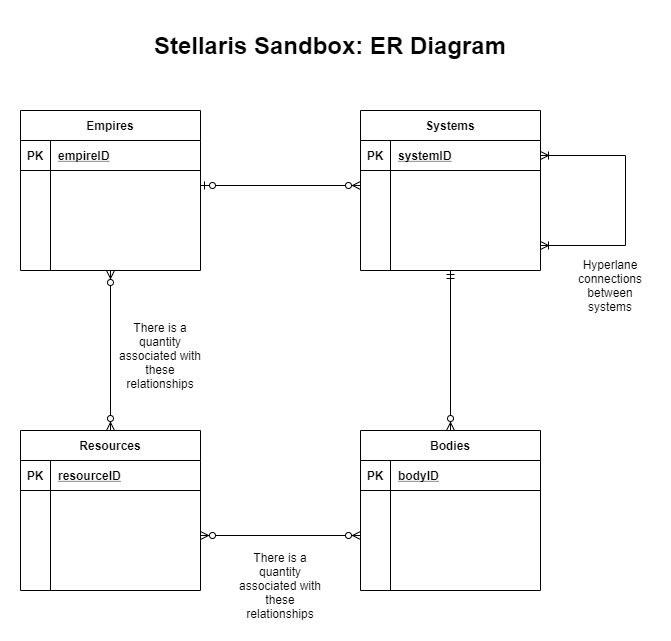
\includegraphics[width=\textwidth]{erd.png}

\newpage
\section{Schema}

\begin{multicols}{2}
\begin{small}
\begin{Verbatim}[commandchars=+\[\]]

Empires(
	+underline[empireID],
	name,
	aggressiveness,
	primaryColor,
	secondaryColor,
	isFallenEmpire)

Systems(
	+underline[systemID],
	name,
	type,
	star1Type,
	star2Type,
	star3Type,
	orbitalRadius,
	theta,
	empireID)

Bodies(
	+underline[bodyID],
	name,
	type,
	planetType,
	orbitalRadius,
	theta,
	systemID)

Resources(
	+underline[resourceID],
	name,
	baseMarketValue,
	color)

Hyperlanes(
	+underline[system1ID],
	+underline[system2ID])

\end{Verbatim}
\columnbreak
\begin{Verbatim}[commandchars=+\[\]]

ResourceStock(
	+underline[empireID],
	+underline[resourceID],
	quantity)

ResourceDeposits(
	+underline[bodyID],
	+underline[resourceID],
	quantity)

\end{Verbatim}
\end{small}
\end{multicols}

\newpage
\section{Screen Captures}

\subsection{Home Page}

\begin{figure}[!ht]
  \caption{Home page, hub slide.}
  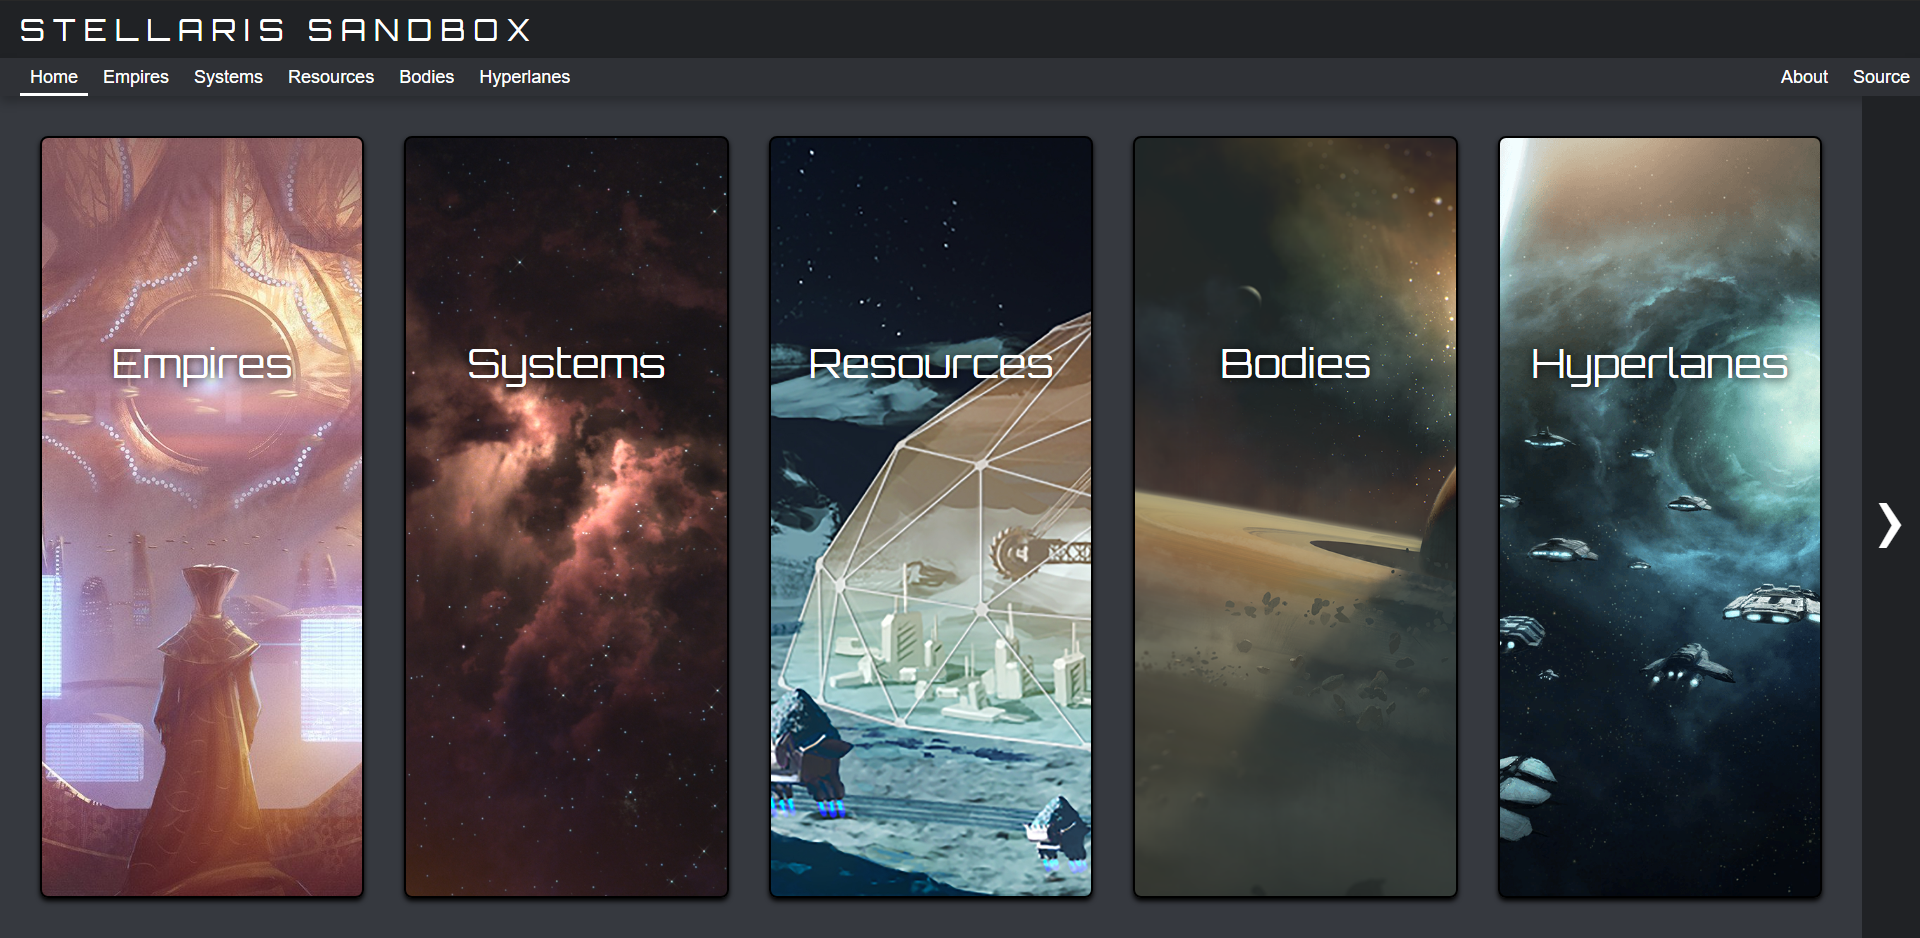
\includegraphics[width=\textwidth]{screenshots/home/home_hub.png}
\end{figure}

\begin{figure}[!ht]
  \caption{Home page, galaxy slide.}
  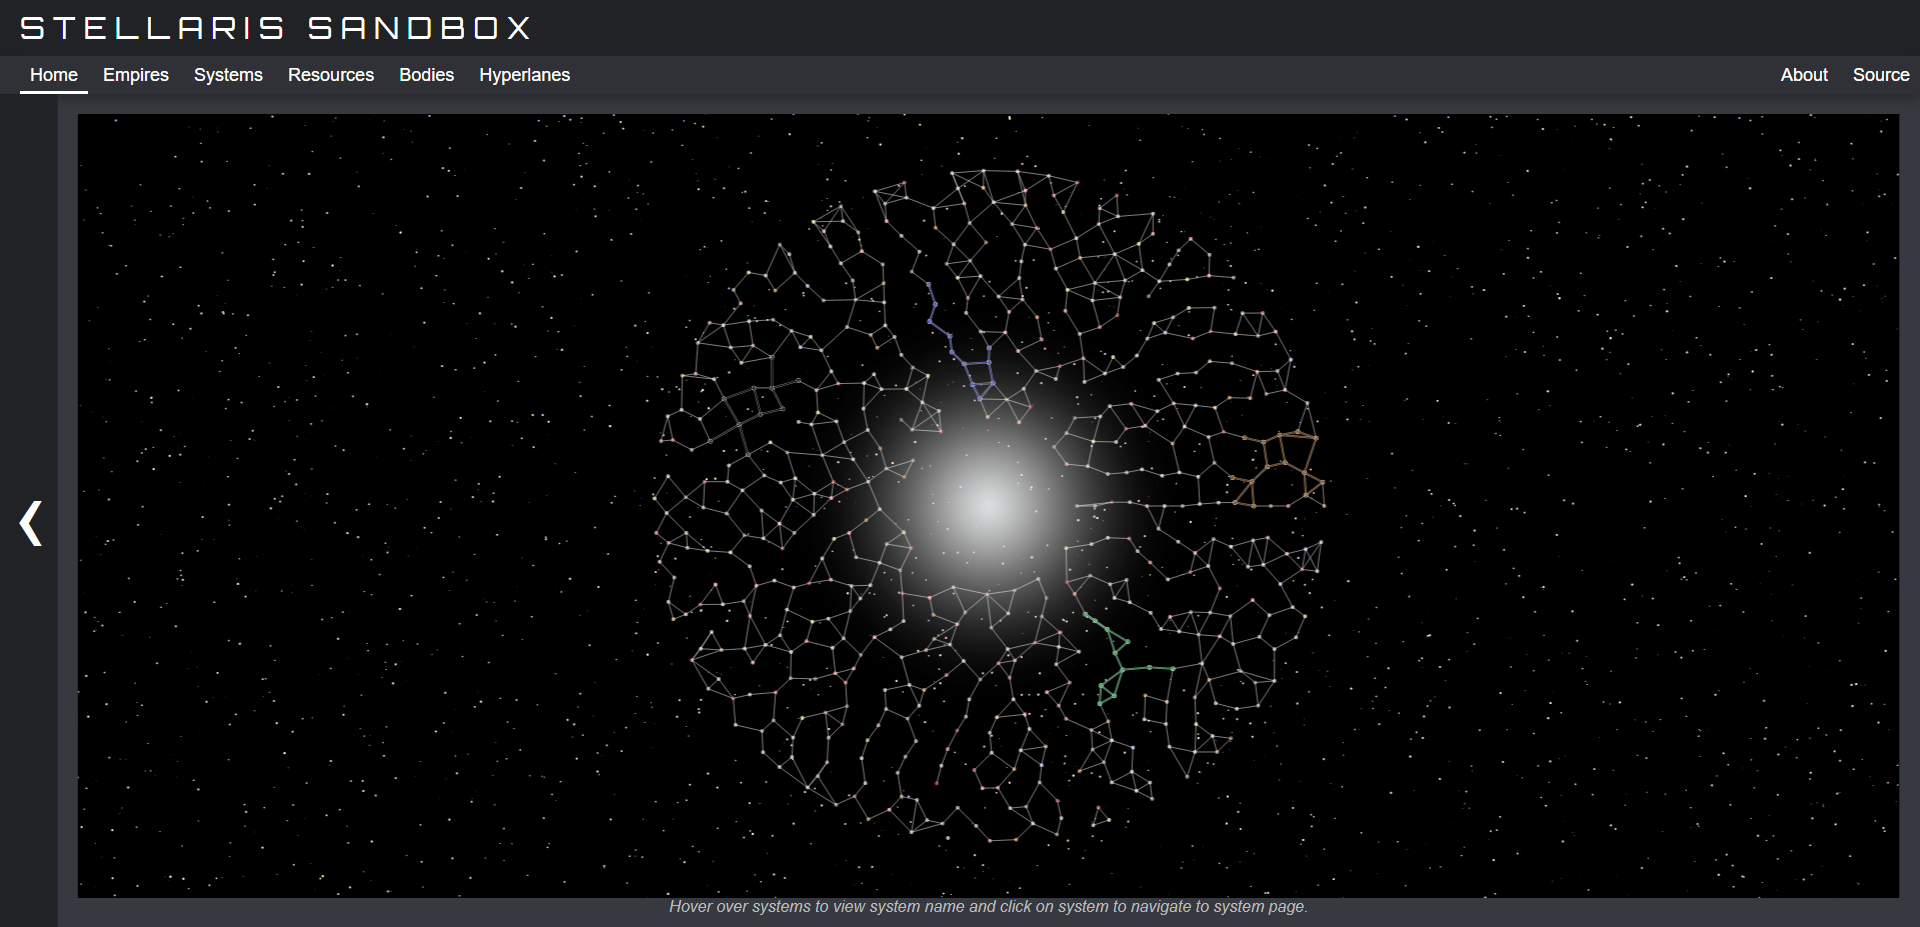
\includegraphics[width=\textwidth]{screenshots/home/home_galaxy.png}
\end{figure}

\newpage
\subsection{Empires}

\begin{figure}[!ht]
  \caption{BROWSE Empires page.}
  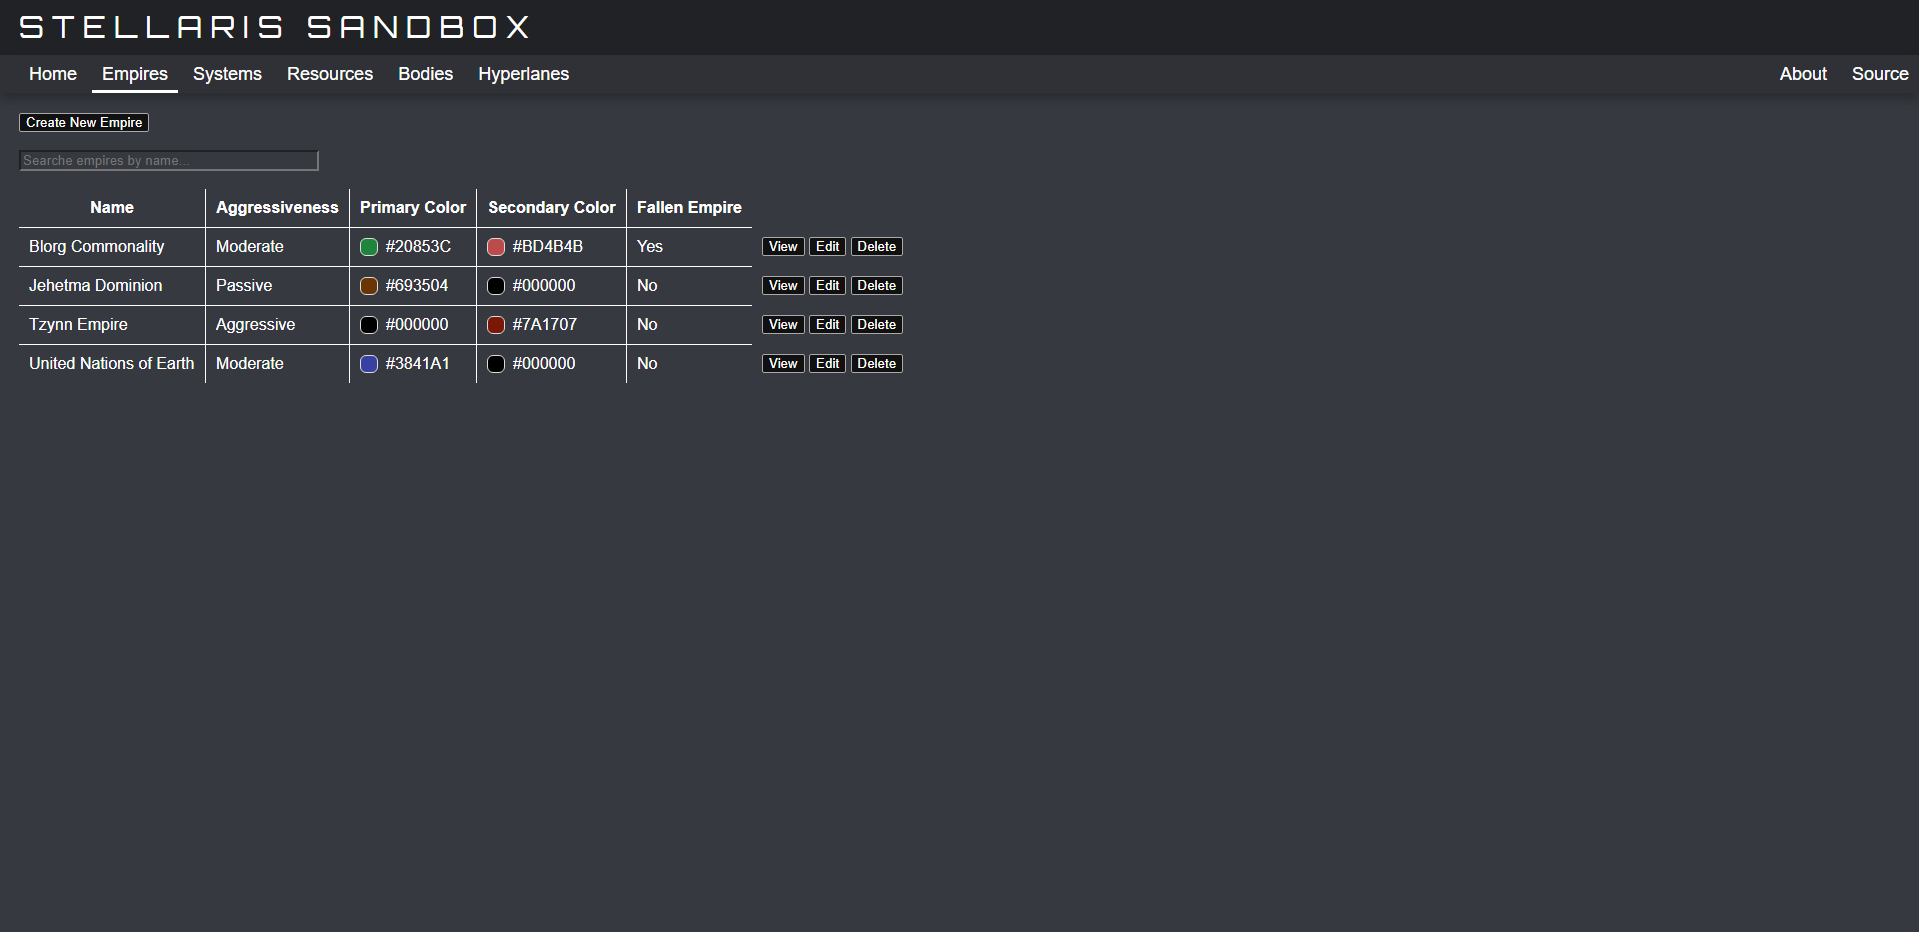
\includegraphics[width=\textwidth]{screenshots/empires/empire_browse.png}
\end{figure}

\begin{figure}[!ht]
  \caption{DELETE Empire page.}
  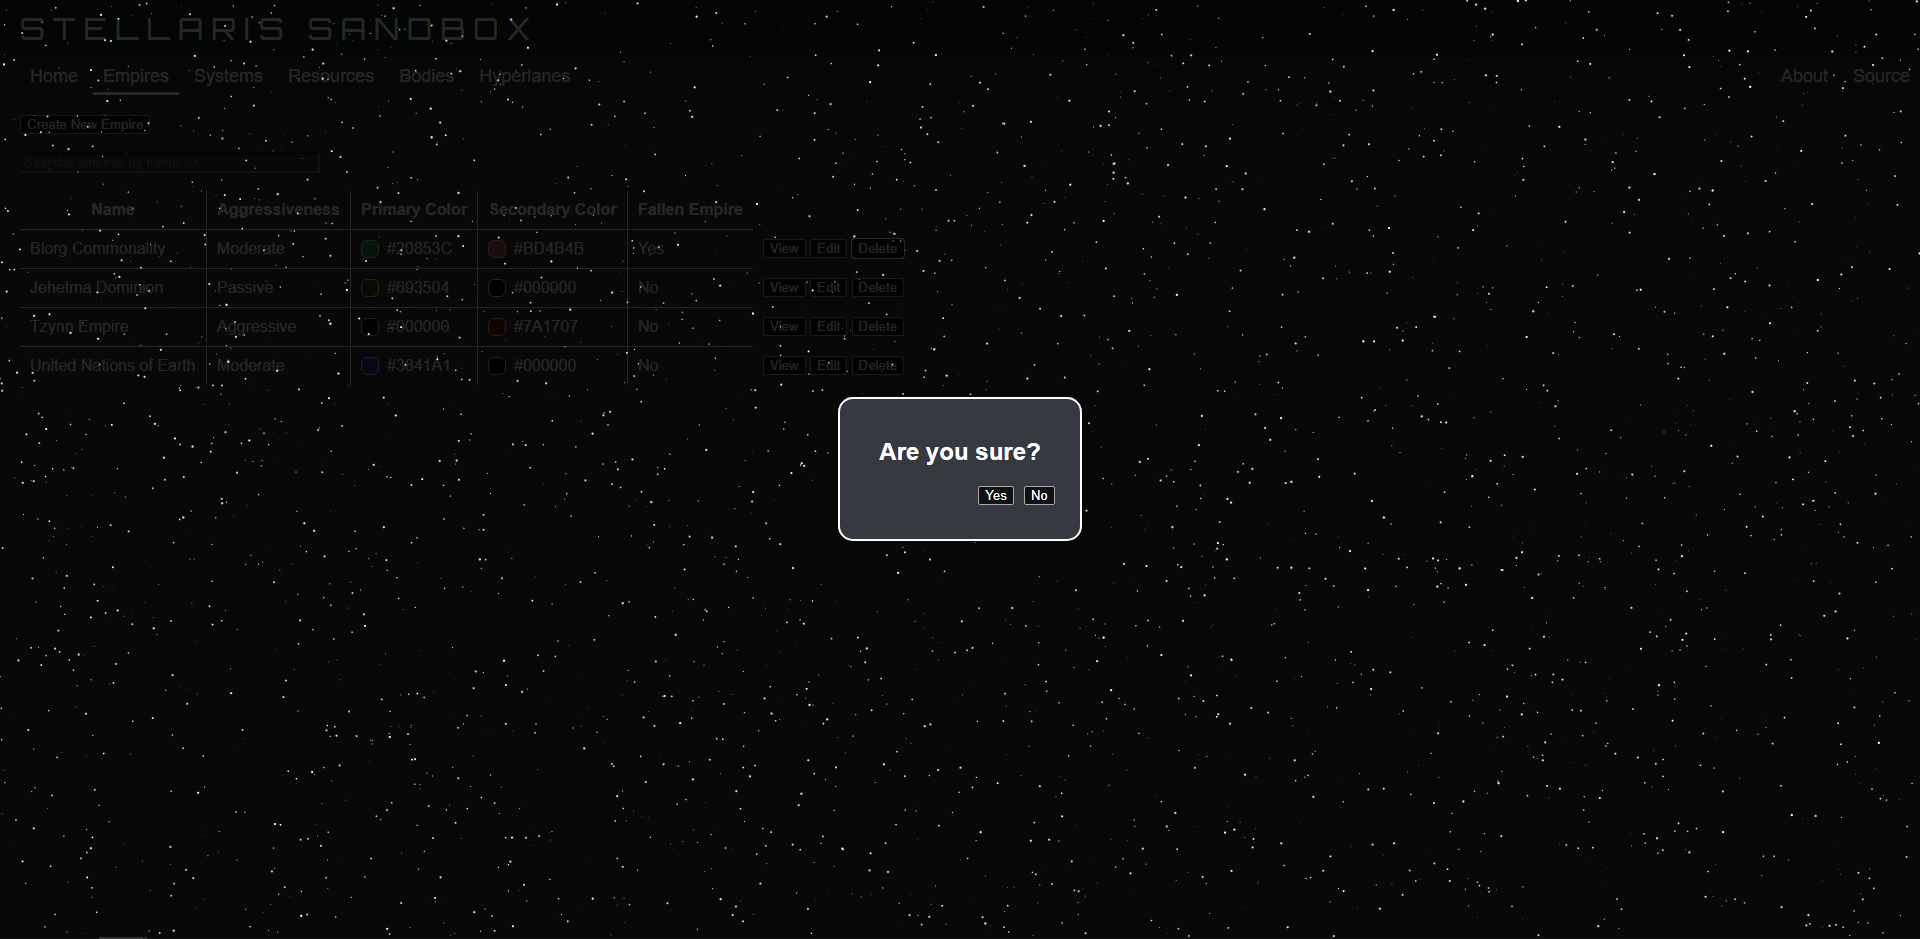
\includegraphics[width=\textwidth]{screenshots/empires/empire_delete.png}
\end{figure}

\begin{figure}[!ht]
  \caption{CREATE Empire page.}
  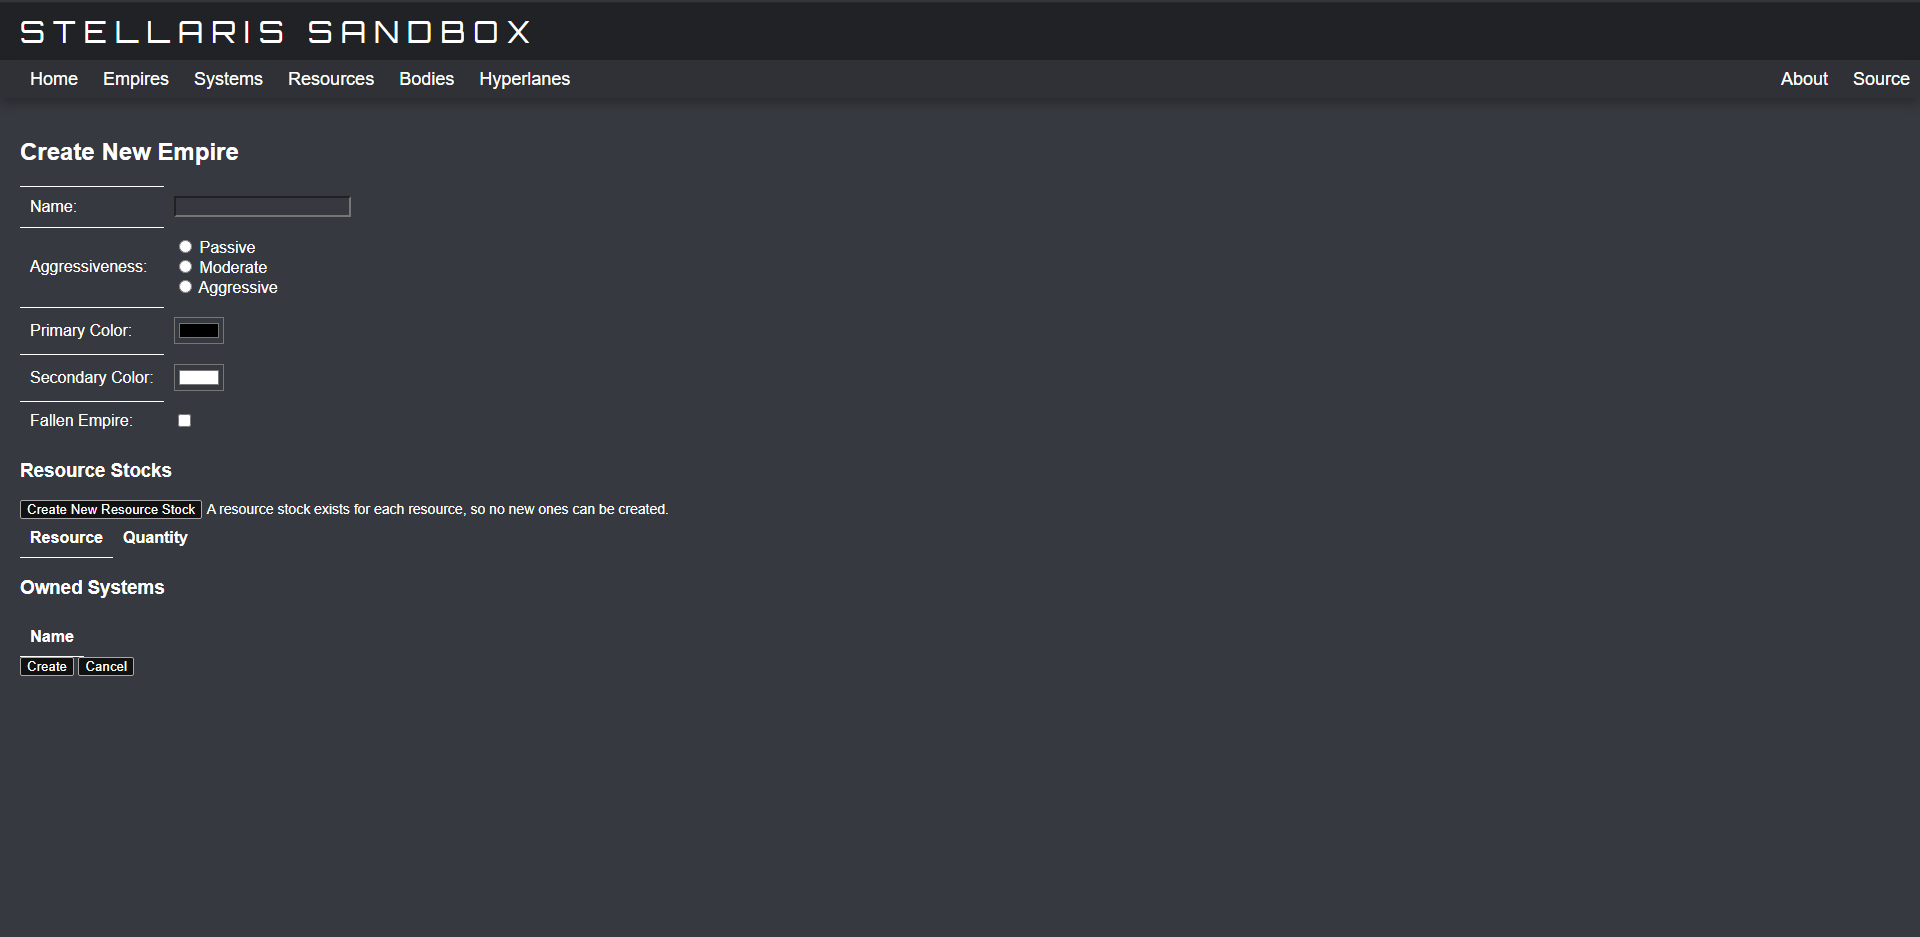
\includegraphics[width=\textwidth]{screenshots/empires/empire_create.png}
\end{figure}

\begin{figure}[!ht]
  \caption{READ Empire page.}
  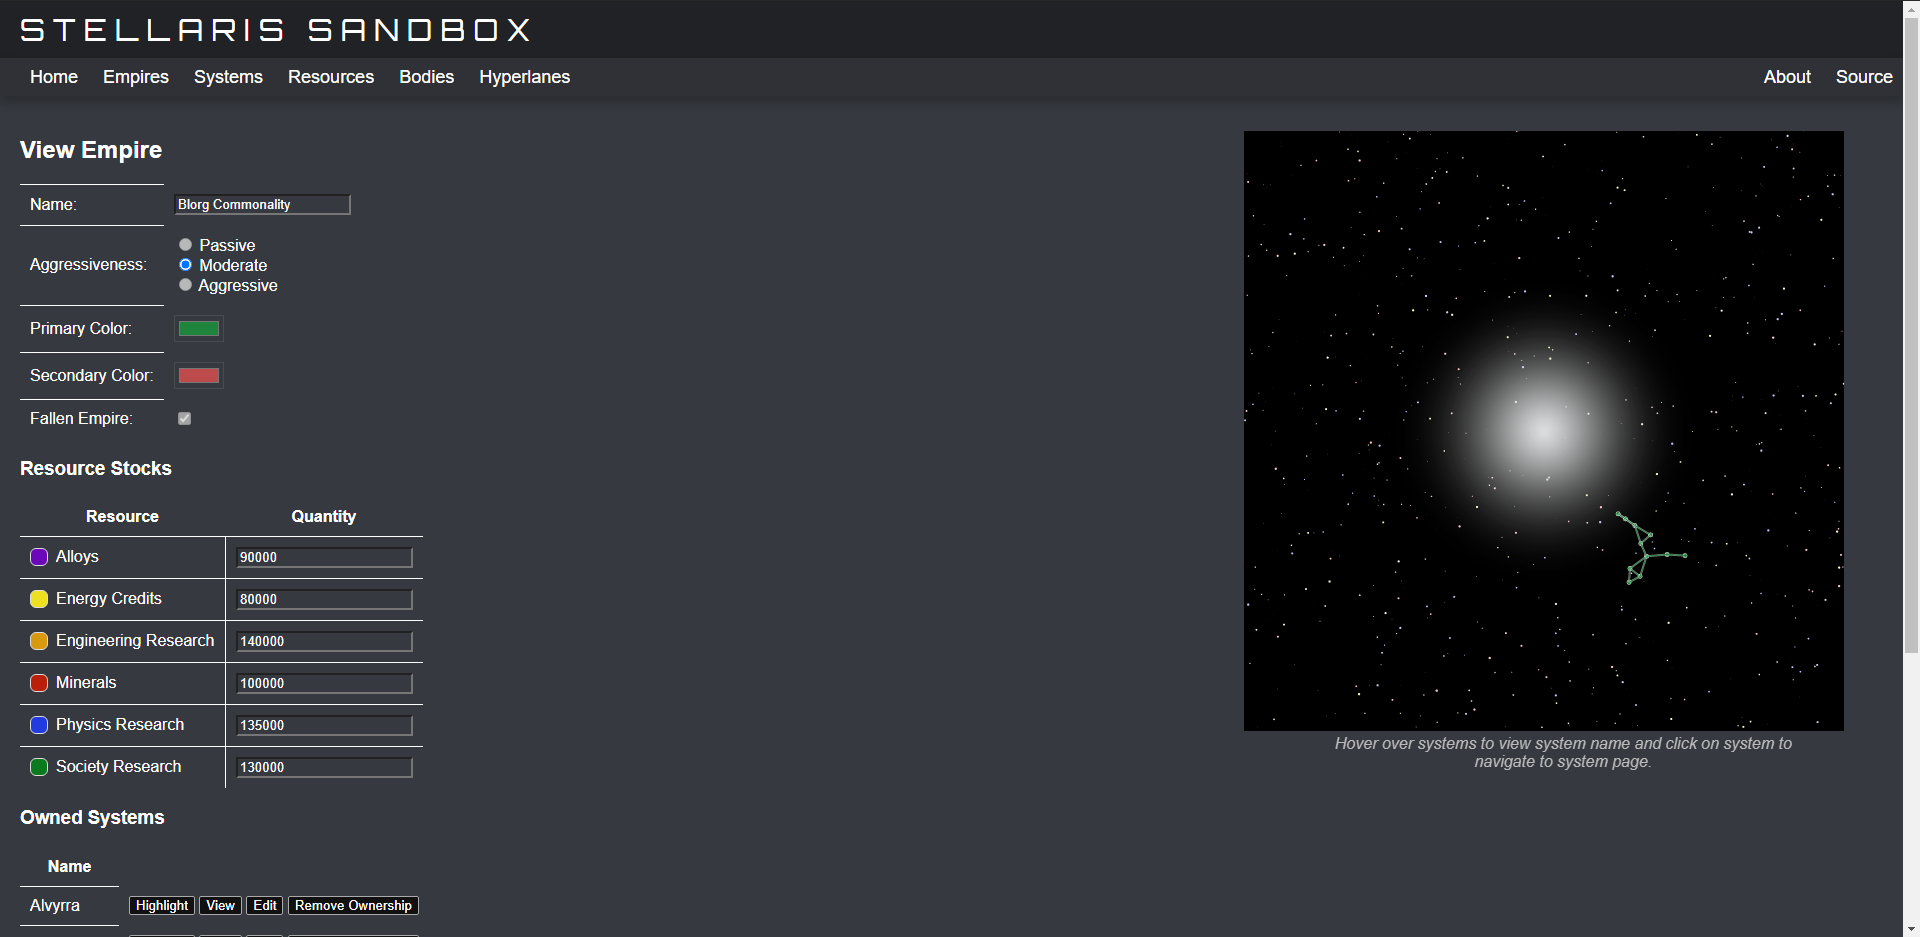
\includegraphics[width=\textwidth]{screenshots/empires/empire_read.png}
\end{figure}

\begin{figure}[!ht]
  \caption{READ/UPDATE Empire page.}
  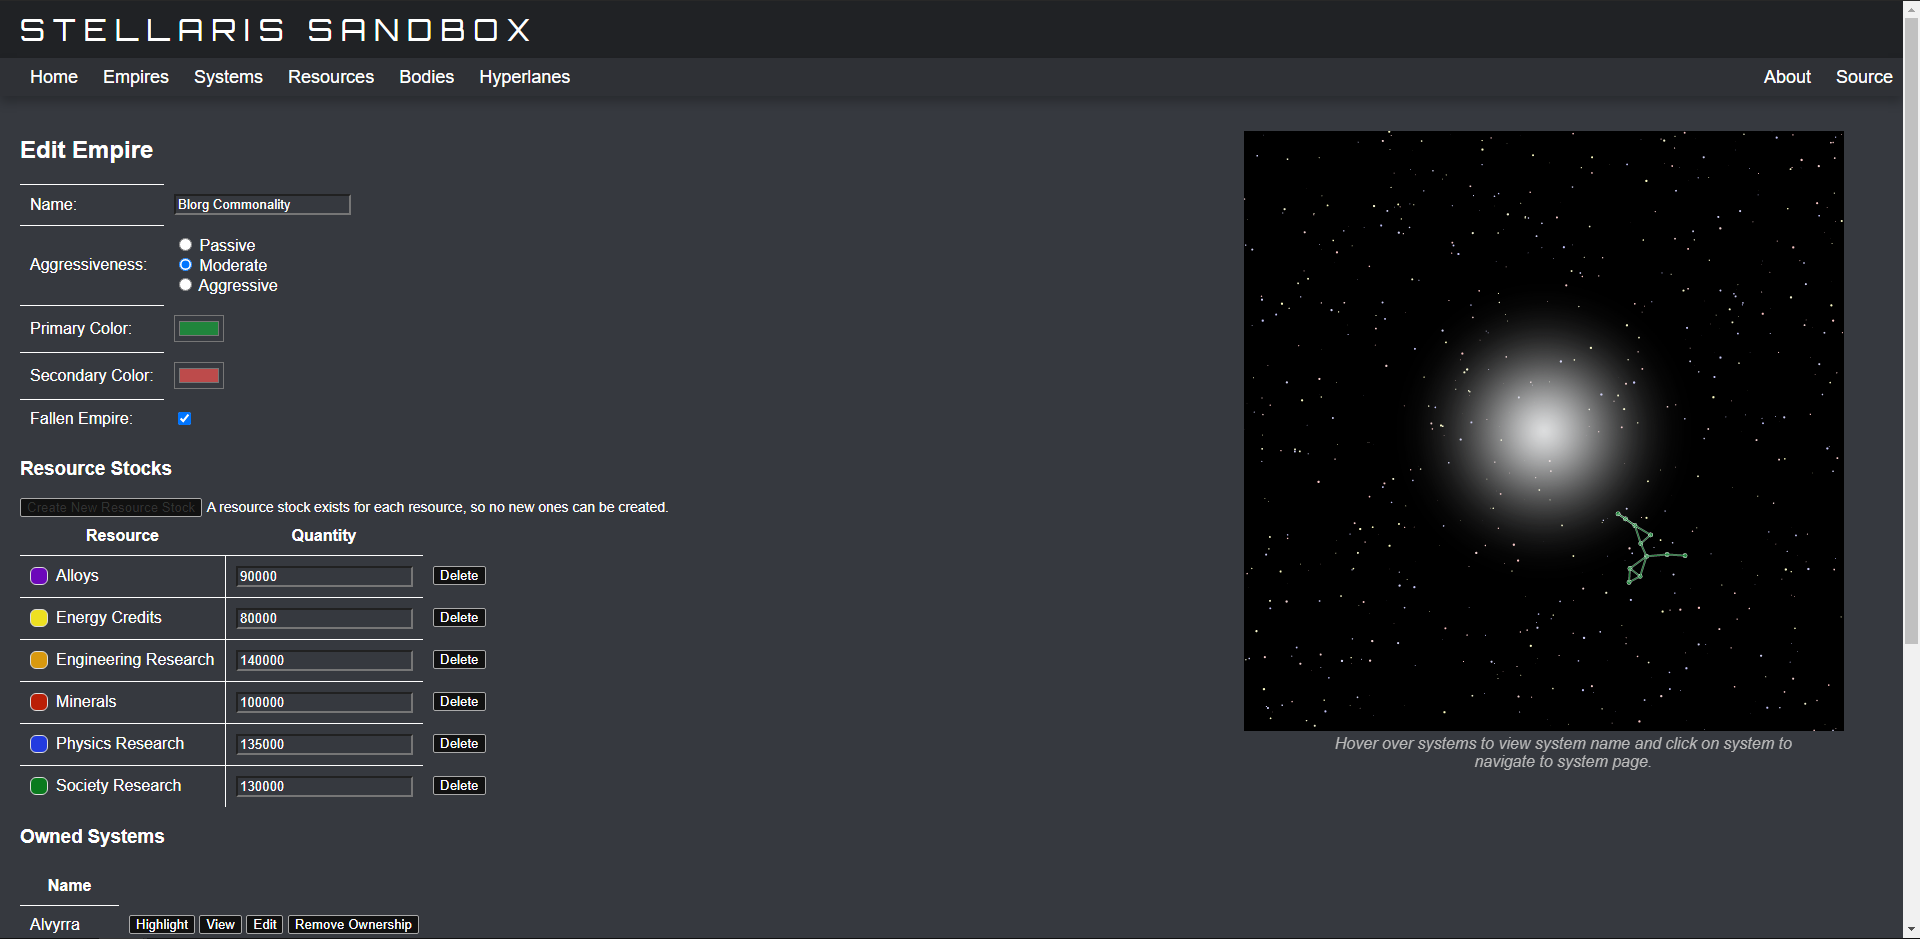
\includegraphics[width=\textwidth]{screenshots/empires/empire_read_update.png}
\end{figure}

\newpage
\subsection{Systems}

\begin{figure}[!ht]
  \caption{BROWSE Systems page.}
  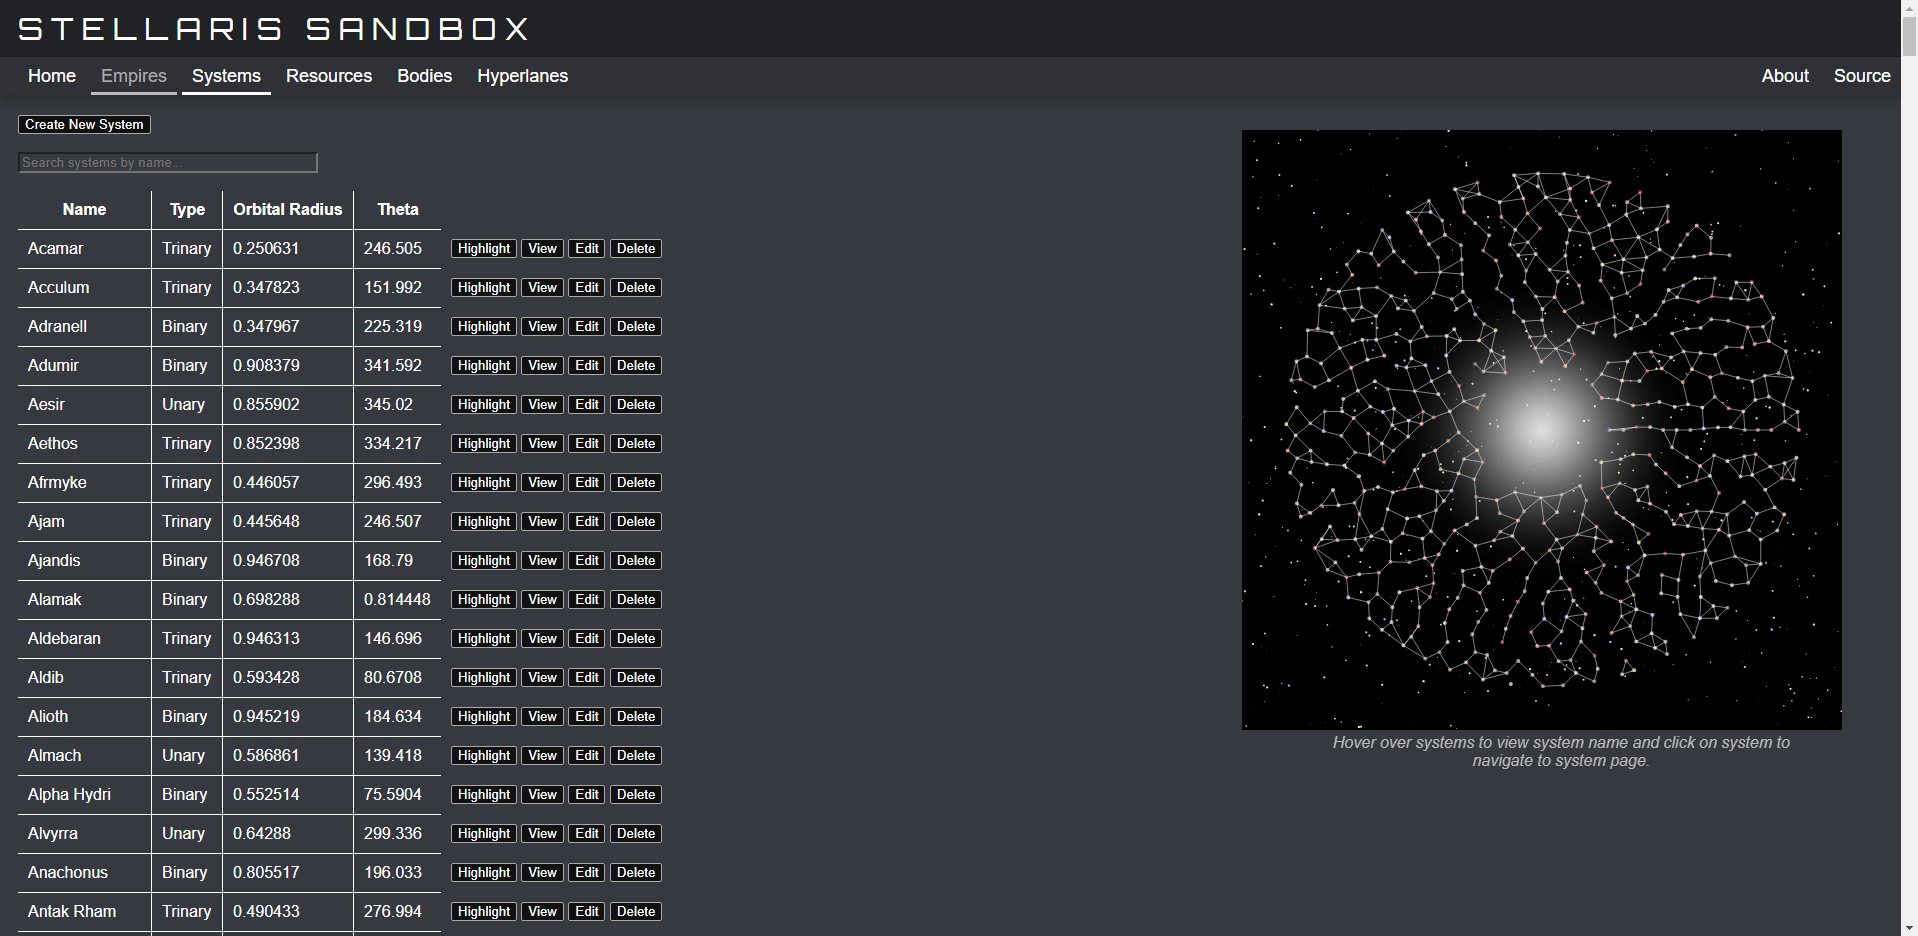
\includegraphics[width=\textwidth]{screenshots/systems/systems_browse.png}
\end{figure}

\begin{figure}[!ht]
  \caption{DELETE System page.}
  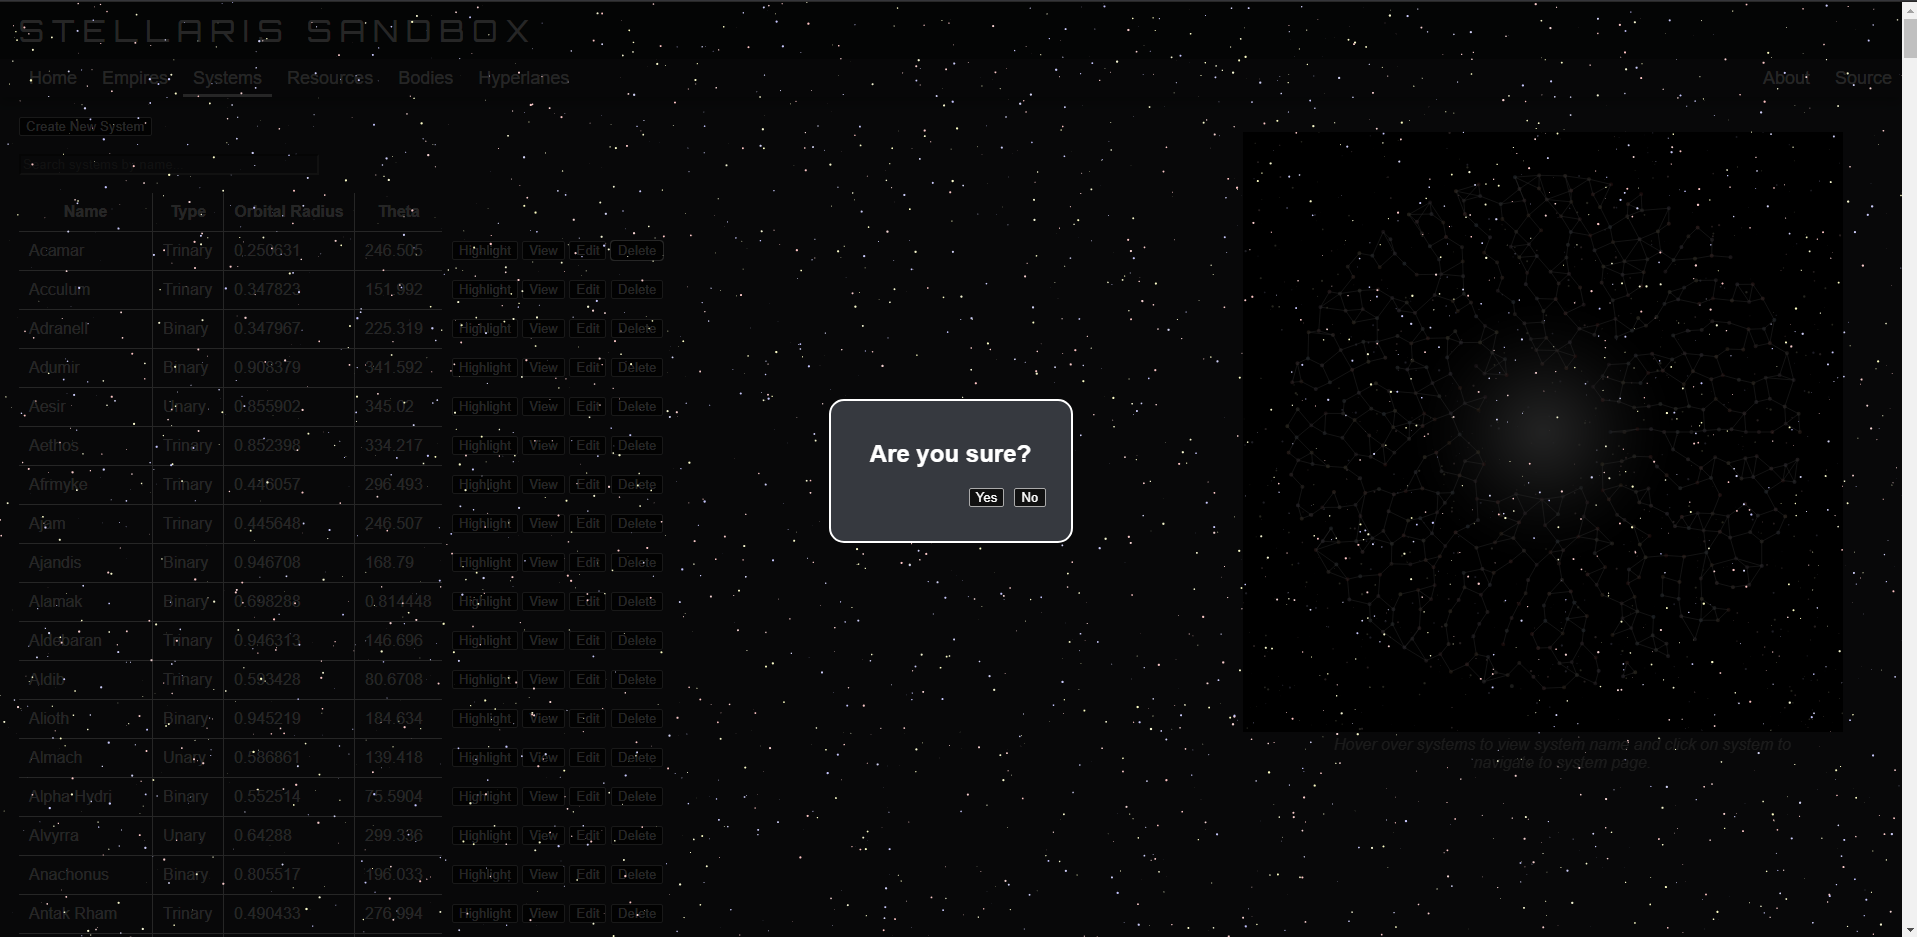
\includegraphics[width=\textwidth]{screenshots/systems/systems_delete.png}
\end{figure}

\begin{figure}[!ht]
  \caption{CREATE System page.}
  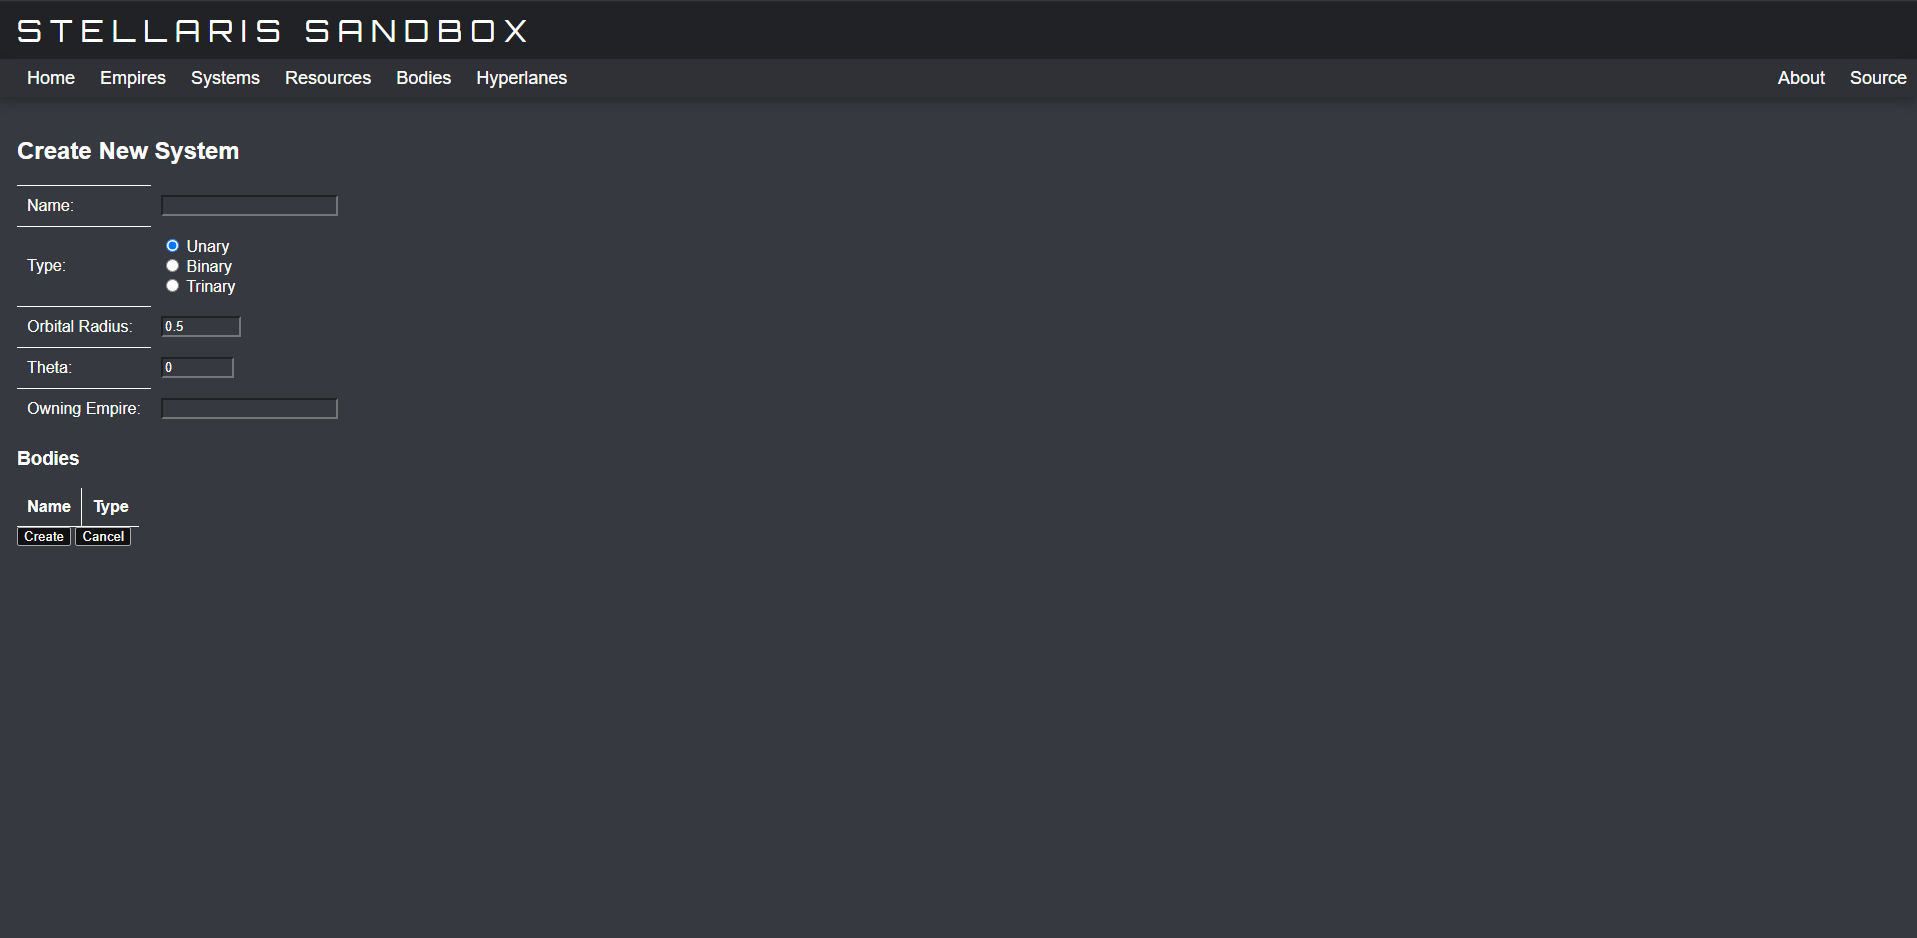
\includegraphics[width=\textwidth]{screenshots/systems/systems_create.png}
\end{figure}

\begin{figure}[!ht]
  \caption{READ System page.}
  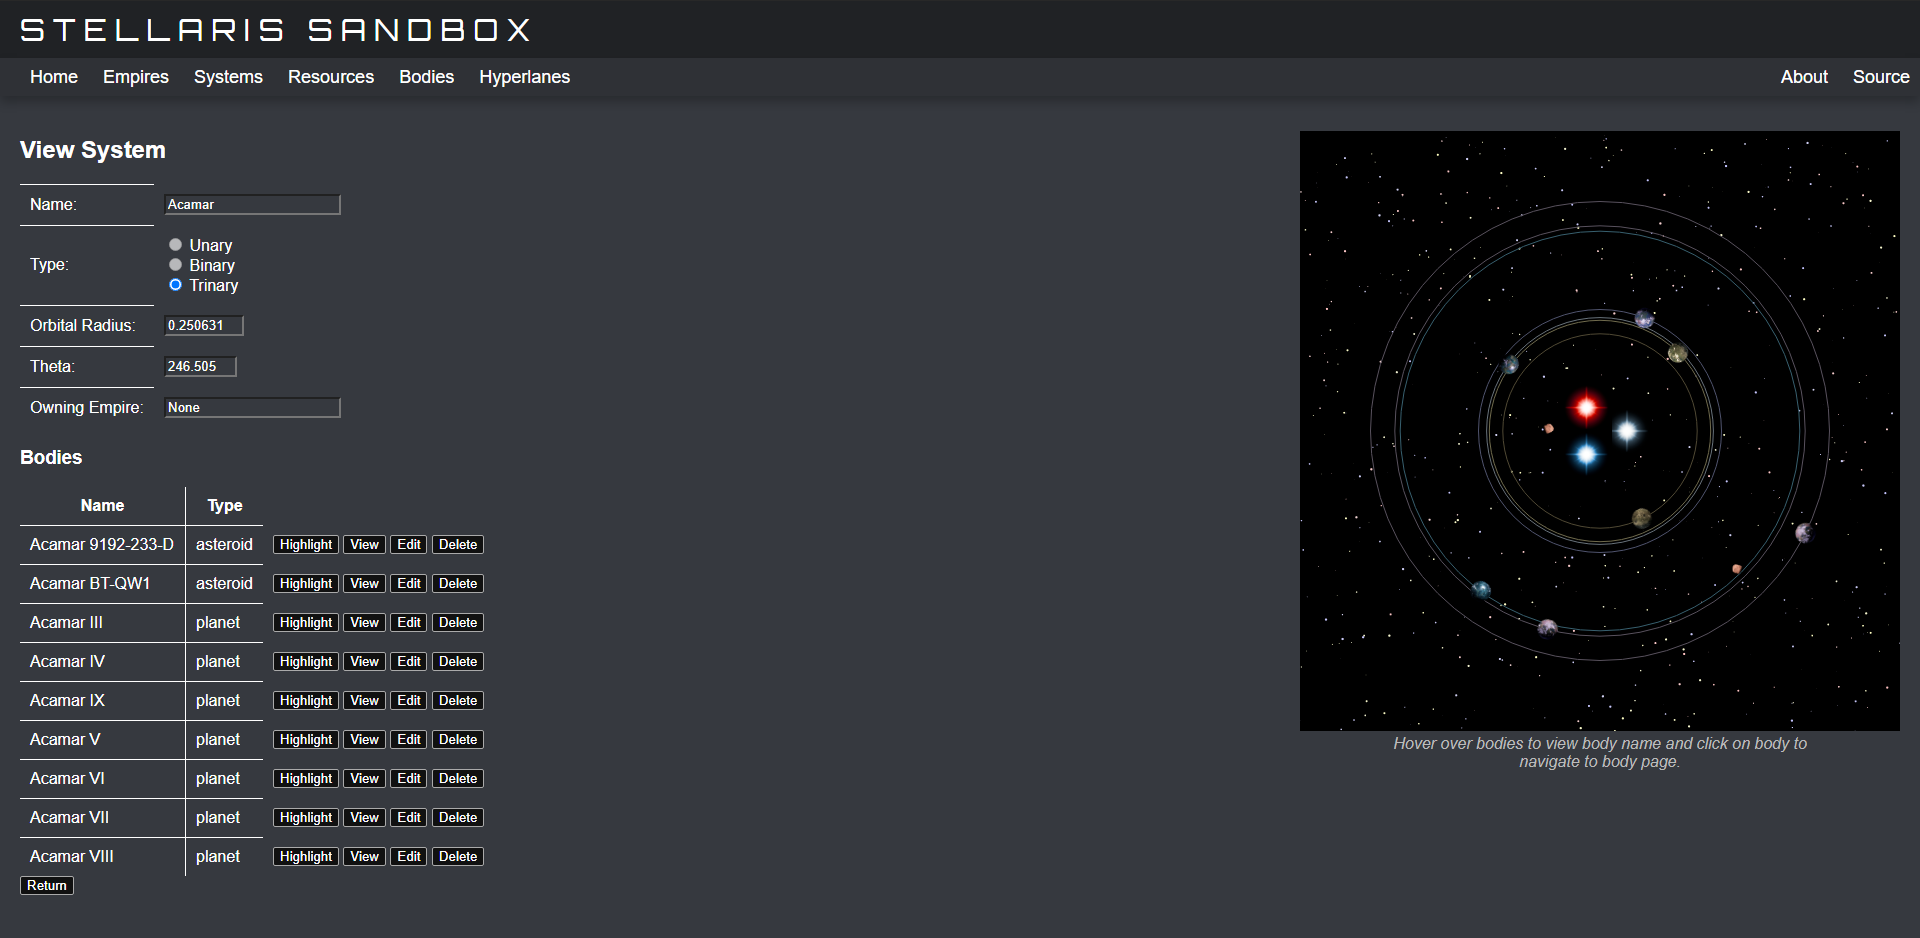
\includegraphics[width=\textwidth]{screenshots/systems/systems_read.png}
\end{figure}

\begin{figure}[!ht]
  \caption{READ/UPDATE System page.}
  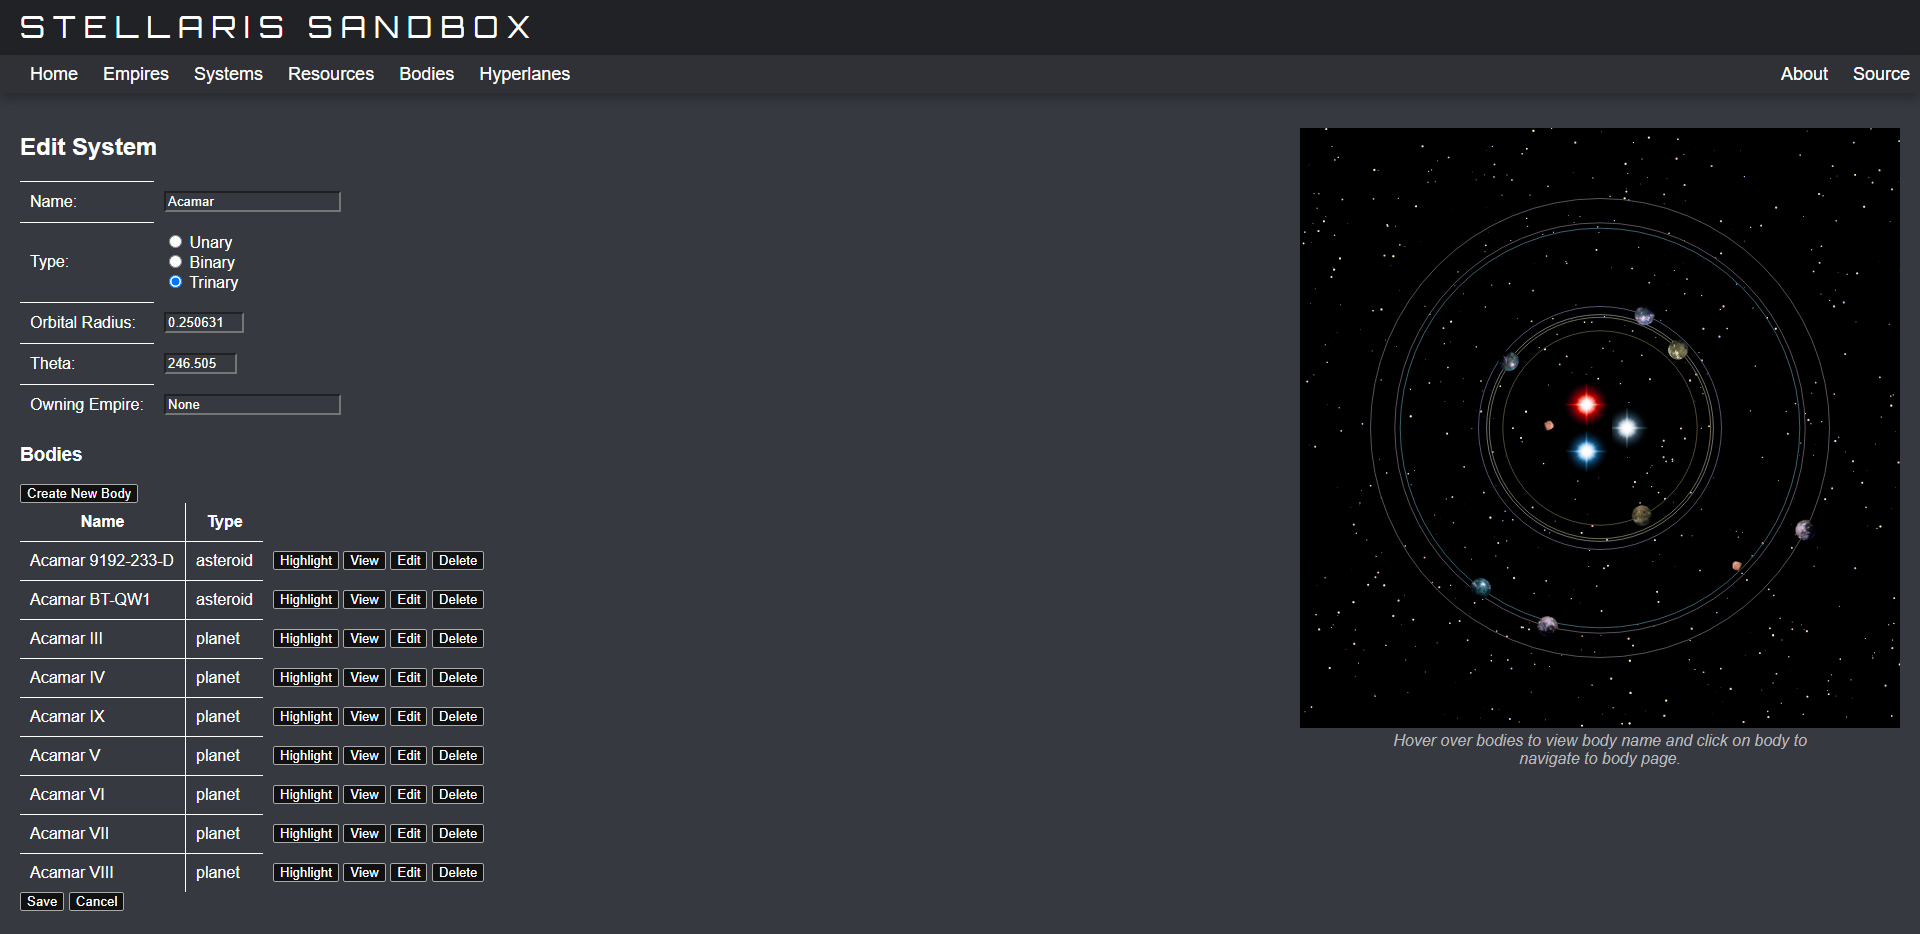
\includegraphics[width=\textwidth]{screenshots/systems/systems_read_update.png}
\end{figure}

\newpage
\subsection{Bodies}

\begin{figure}[!ht]
  \caption{BROWSE Bodies page.}
  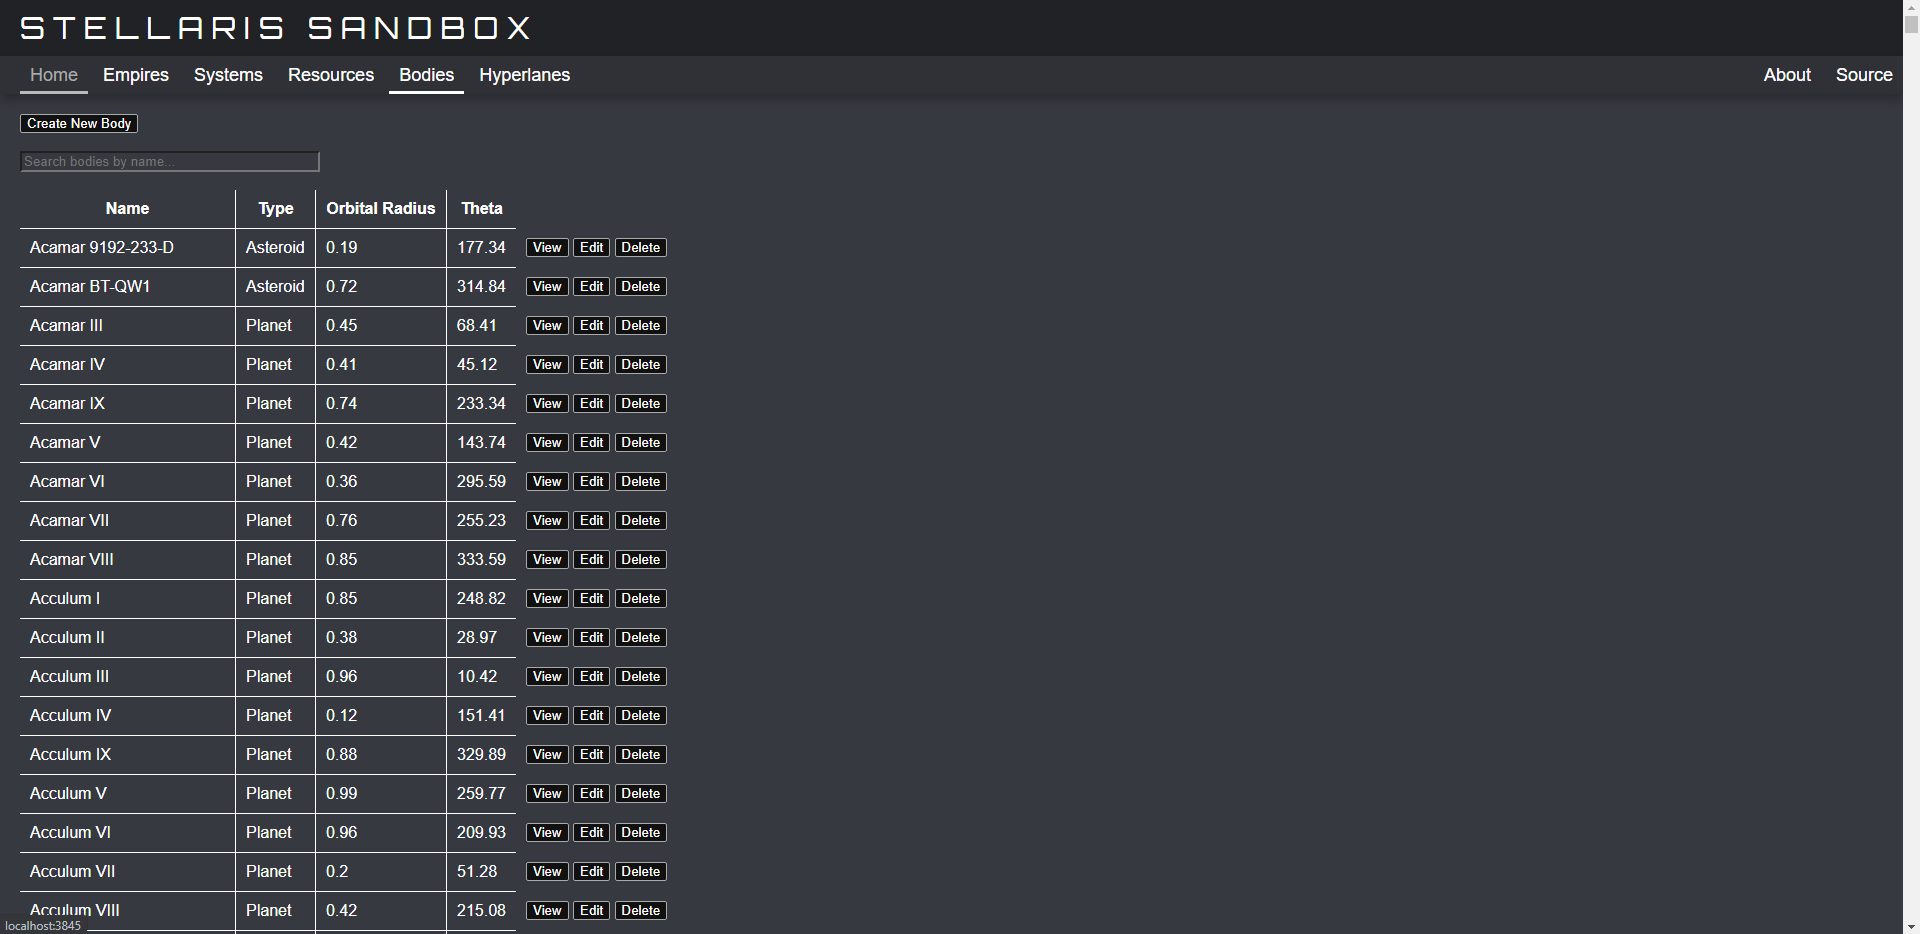
\includegraphics[width=\textwidth]{screenshots/bodies/bodies_browse.png}
\end{figure}

\begin{figure}[!ht]
  \caption{DELETE Body page.}
  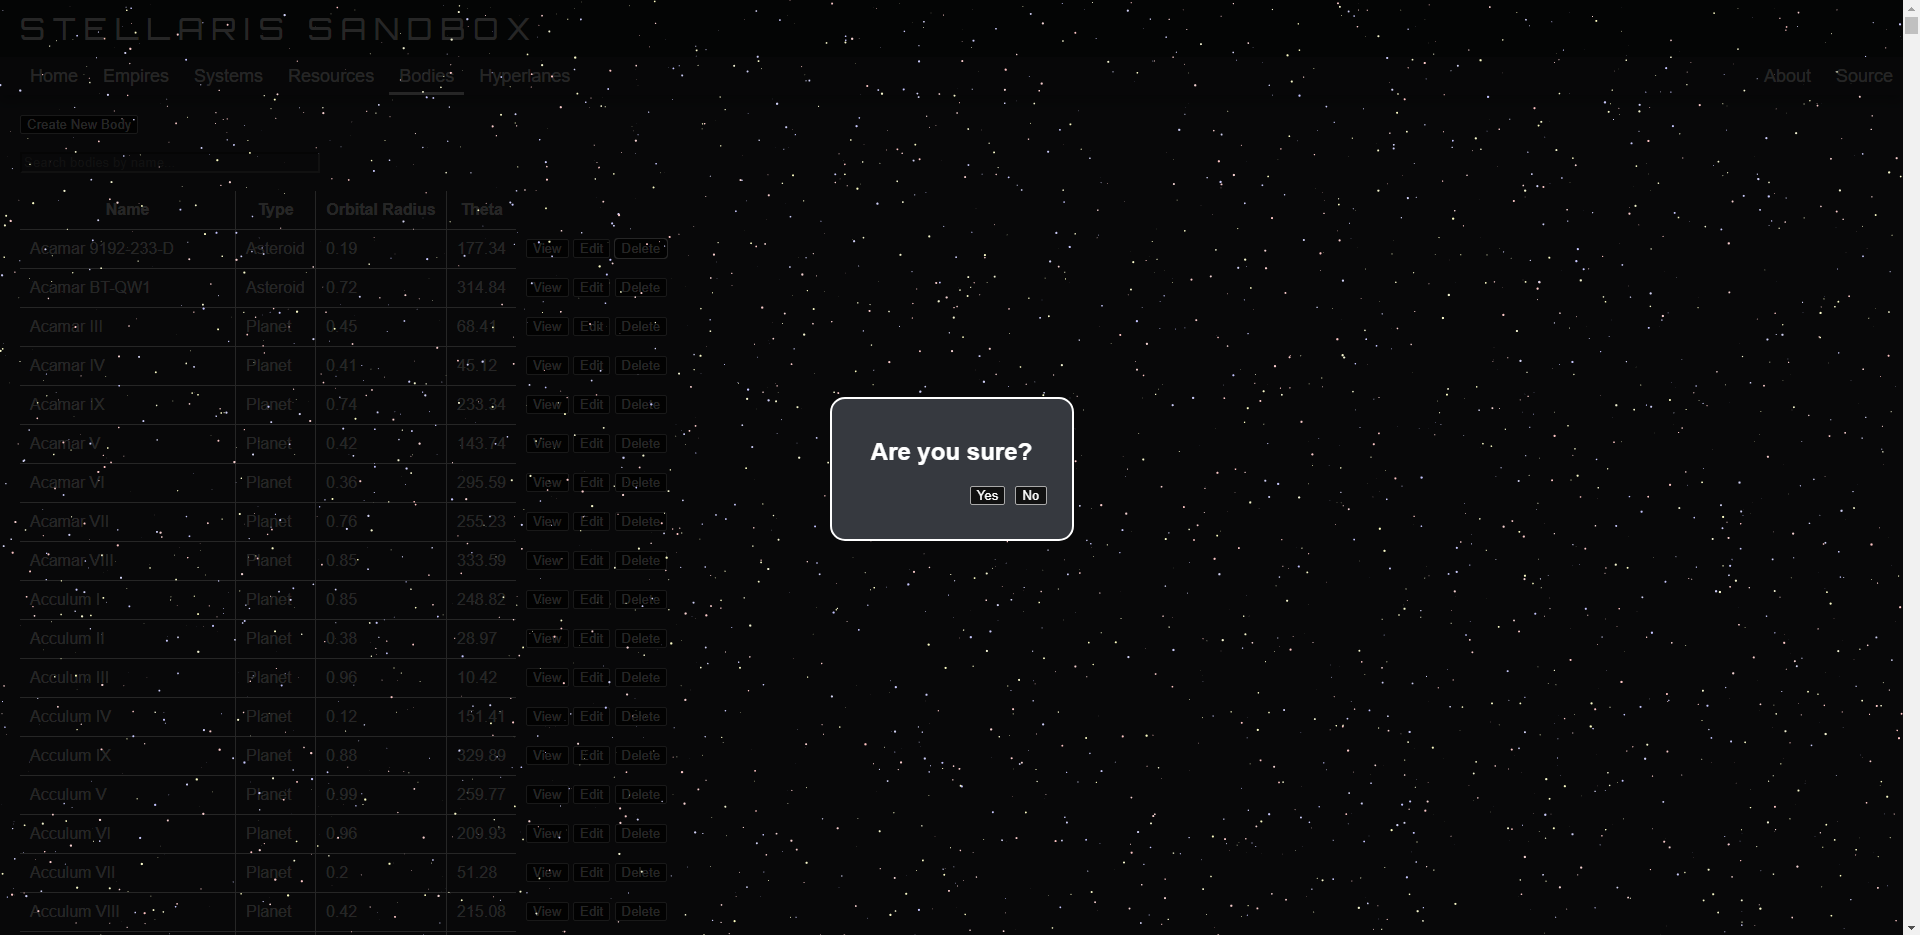
\includegraphics[width=\textwidth]{screenshots/bodies/bodies_delete.png}
\end{figure}

\begin{figure}[!ht]
  \caption{CREATE Body page.}
  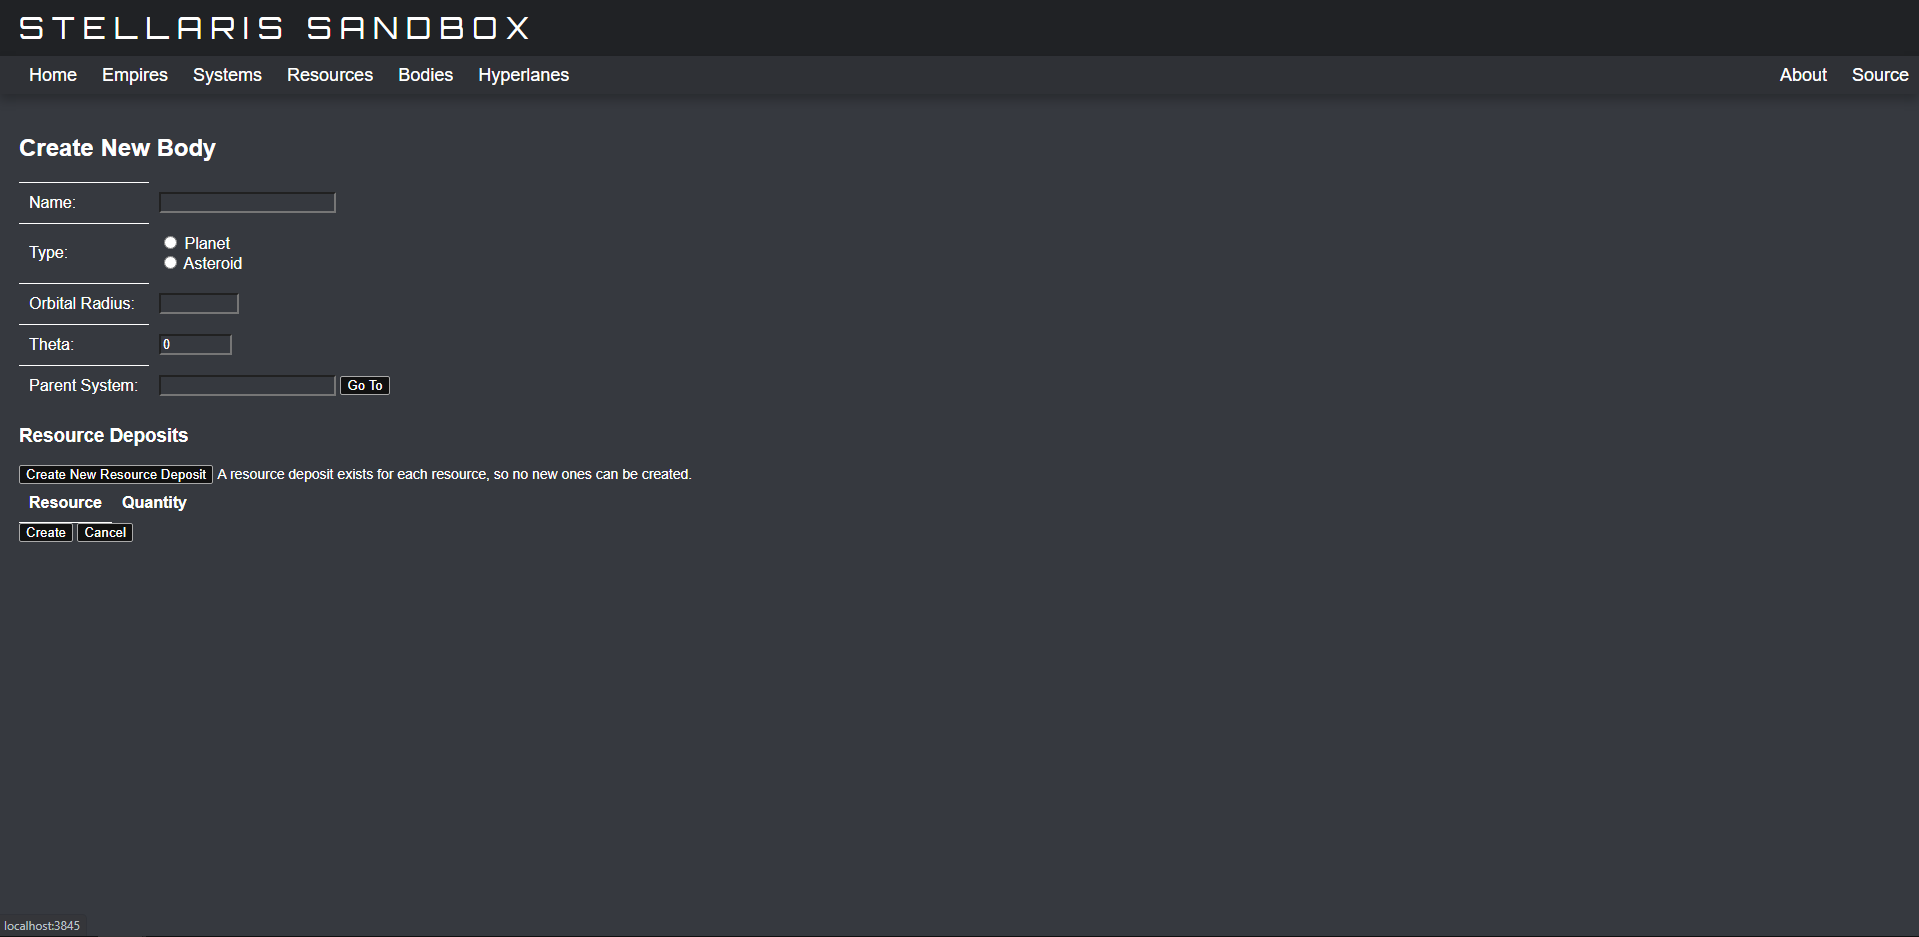
\includegraphics[width=\textwidth]{screenshots/bodies/bodies_create.png}
\end{figure}

\begin{figure}[!ht]
  \caption{READ Body page.}
  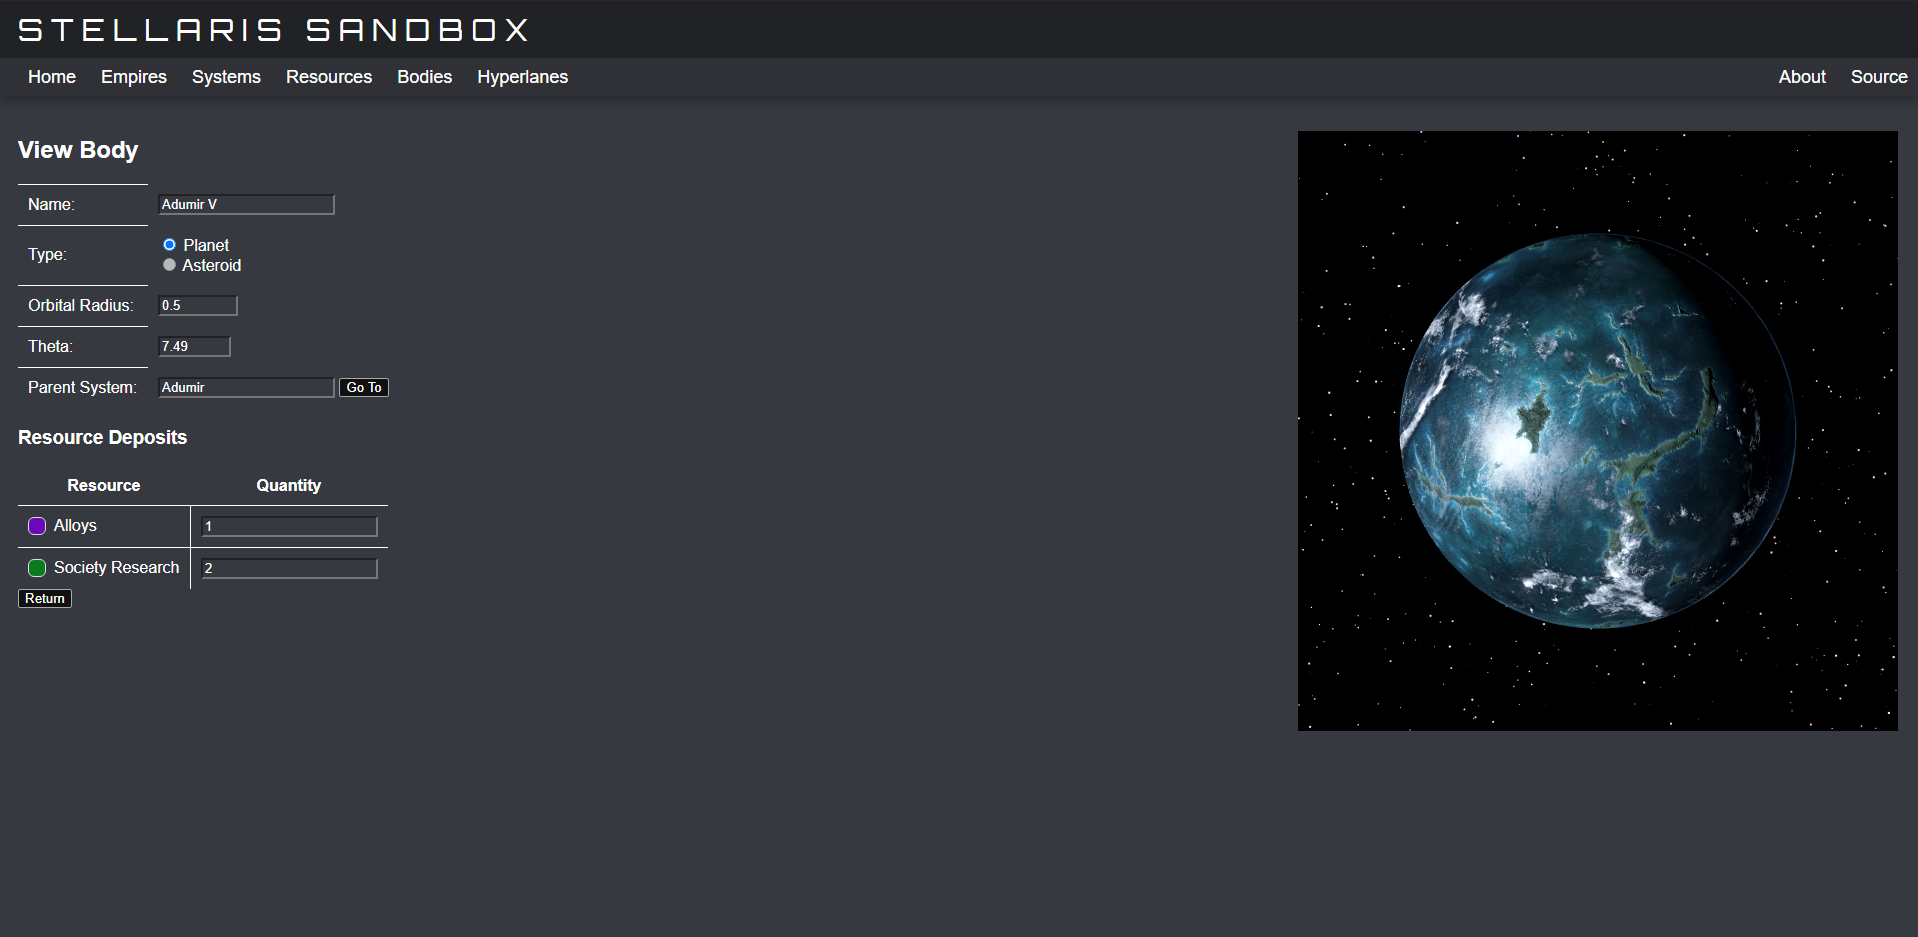
\includegraphics[width=\textwidth]{screenshots/bodies/bodies_read.png}
\end{figure}

\begin{figure}[!ht]
  \caption{READ/UPDATE Body page.}
  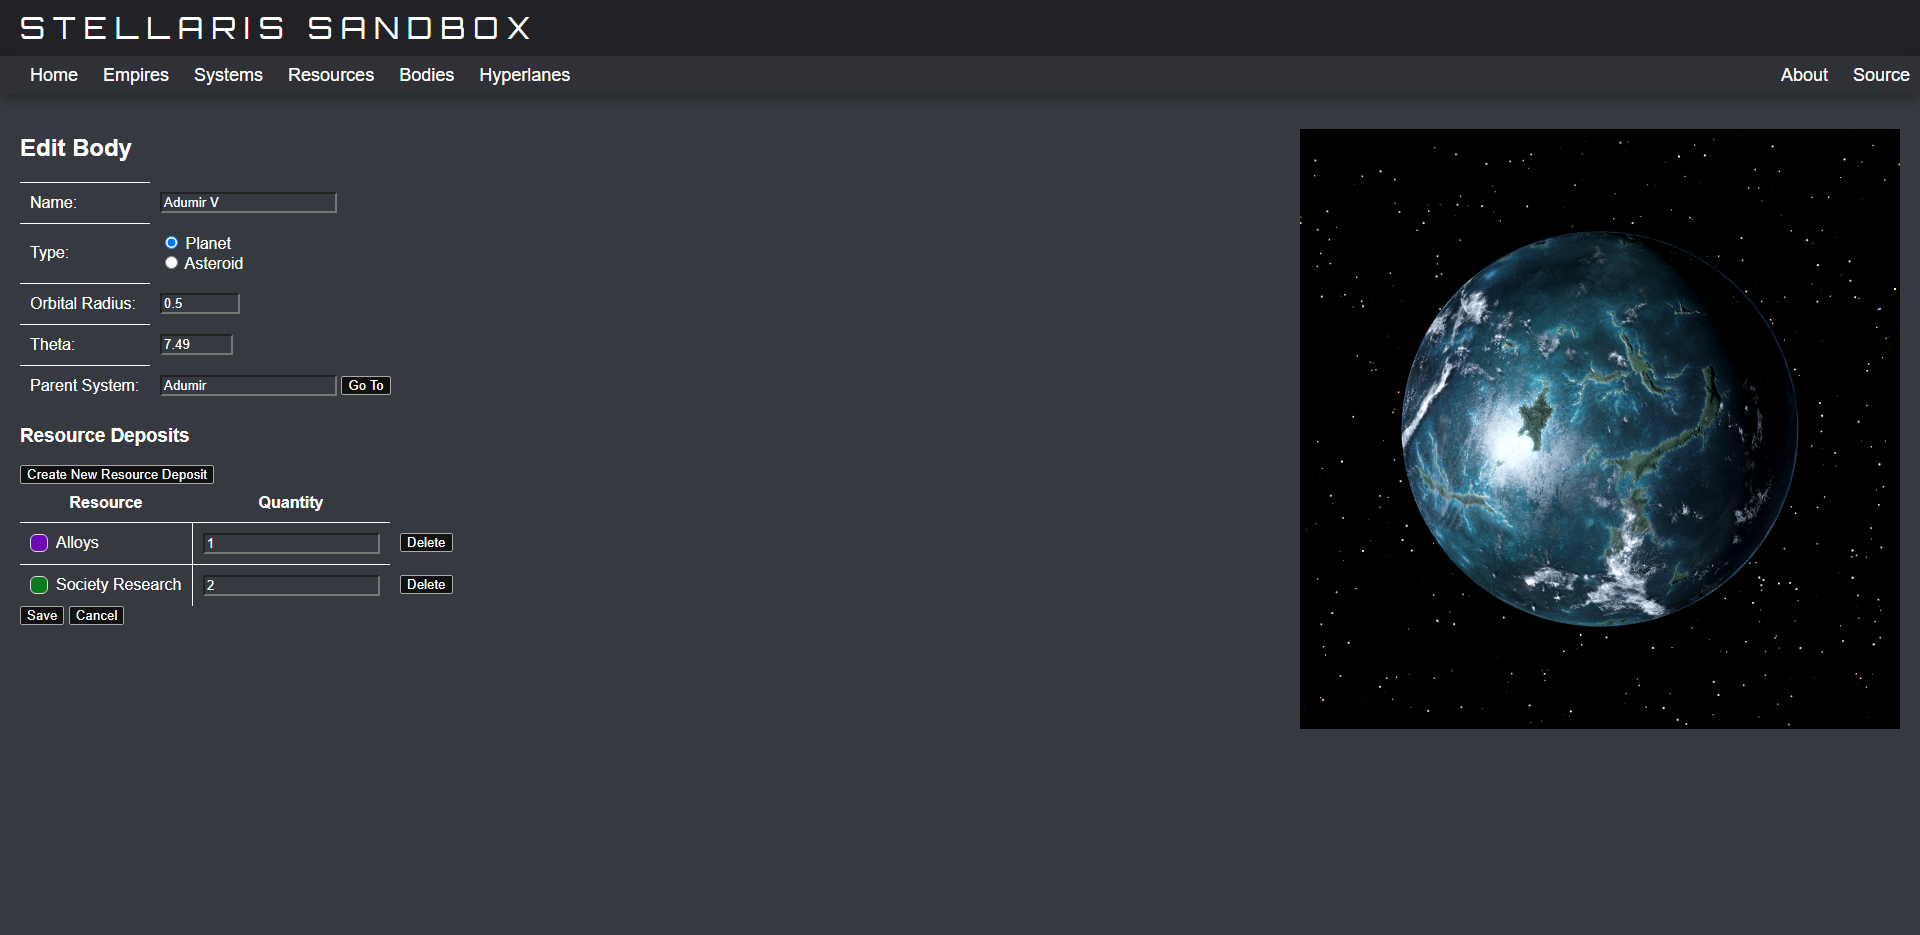
\includegraphics[width=\textwidth]{screenshots/bodies/bodies_read_update.png}
\end{figure}

\newpage
\subsection{Resources}

\begin{figure}[!ht]
  \caption{BROWSE Resources page.}
  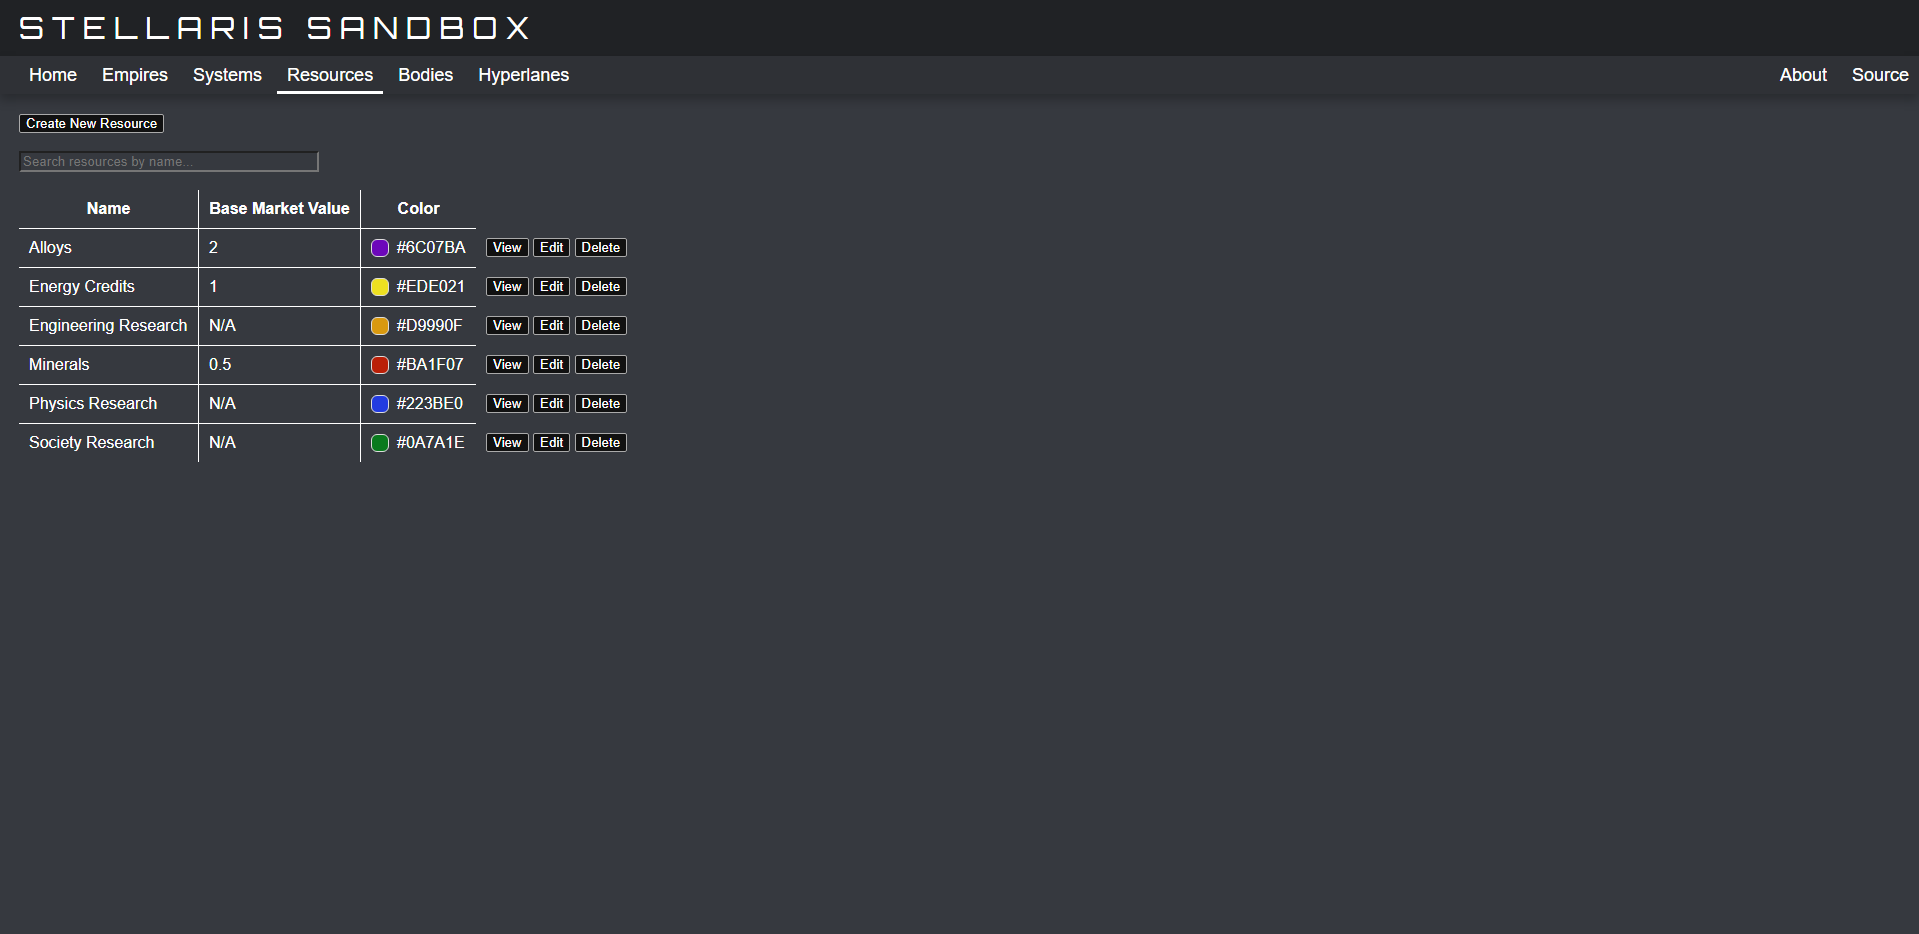
\includegraphics[width=\textwidth]{screenshots/resources/resources_browse.png}
\end{figure}

\begin{figure}[!ht]
  \caption{DELETE Resource page.}
  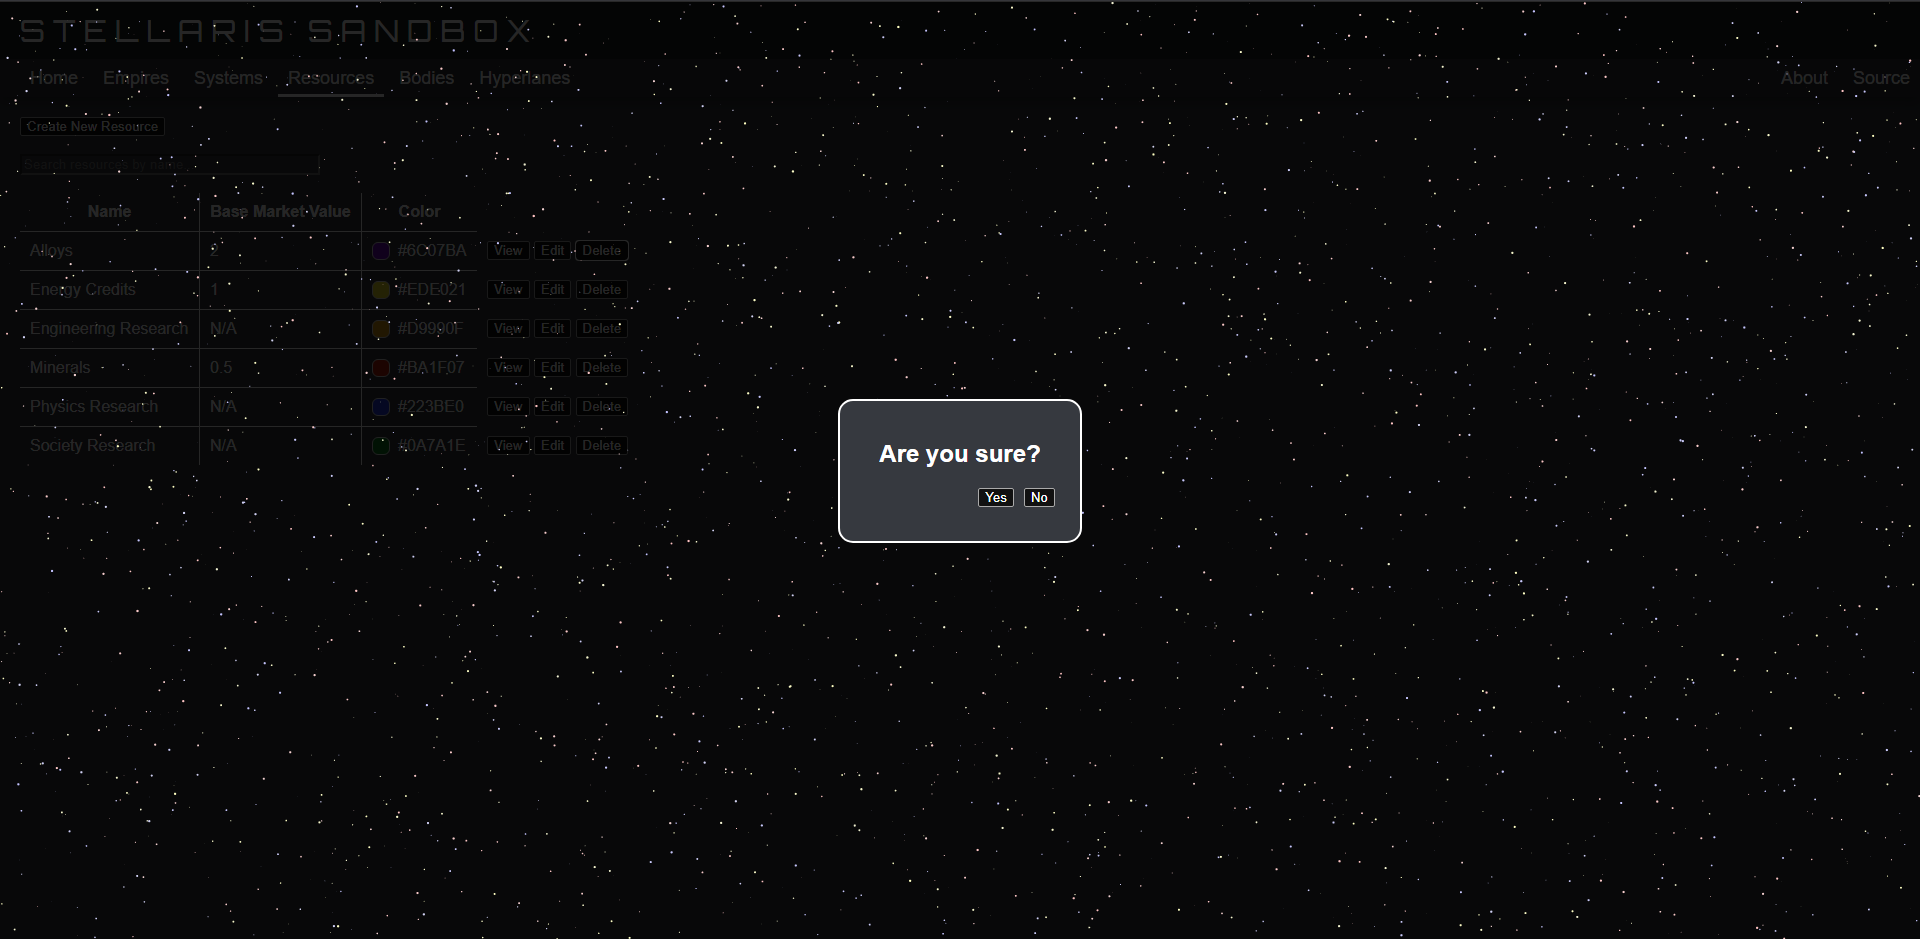
\includegraphics[width=\textwidth]{screenshots/resources/resources_delete.png}
\end{figure}

\begin{figure}[!ht]
  \caption{CREATE Resource page.}
  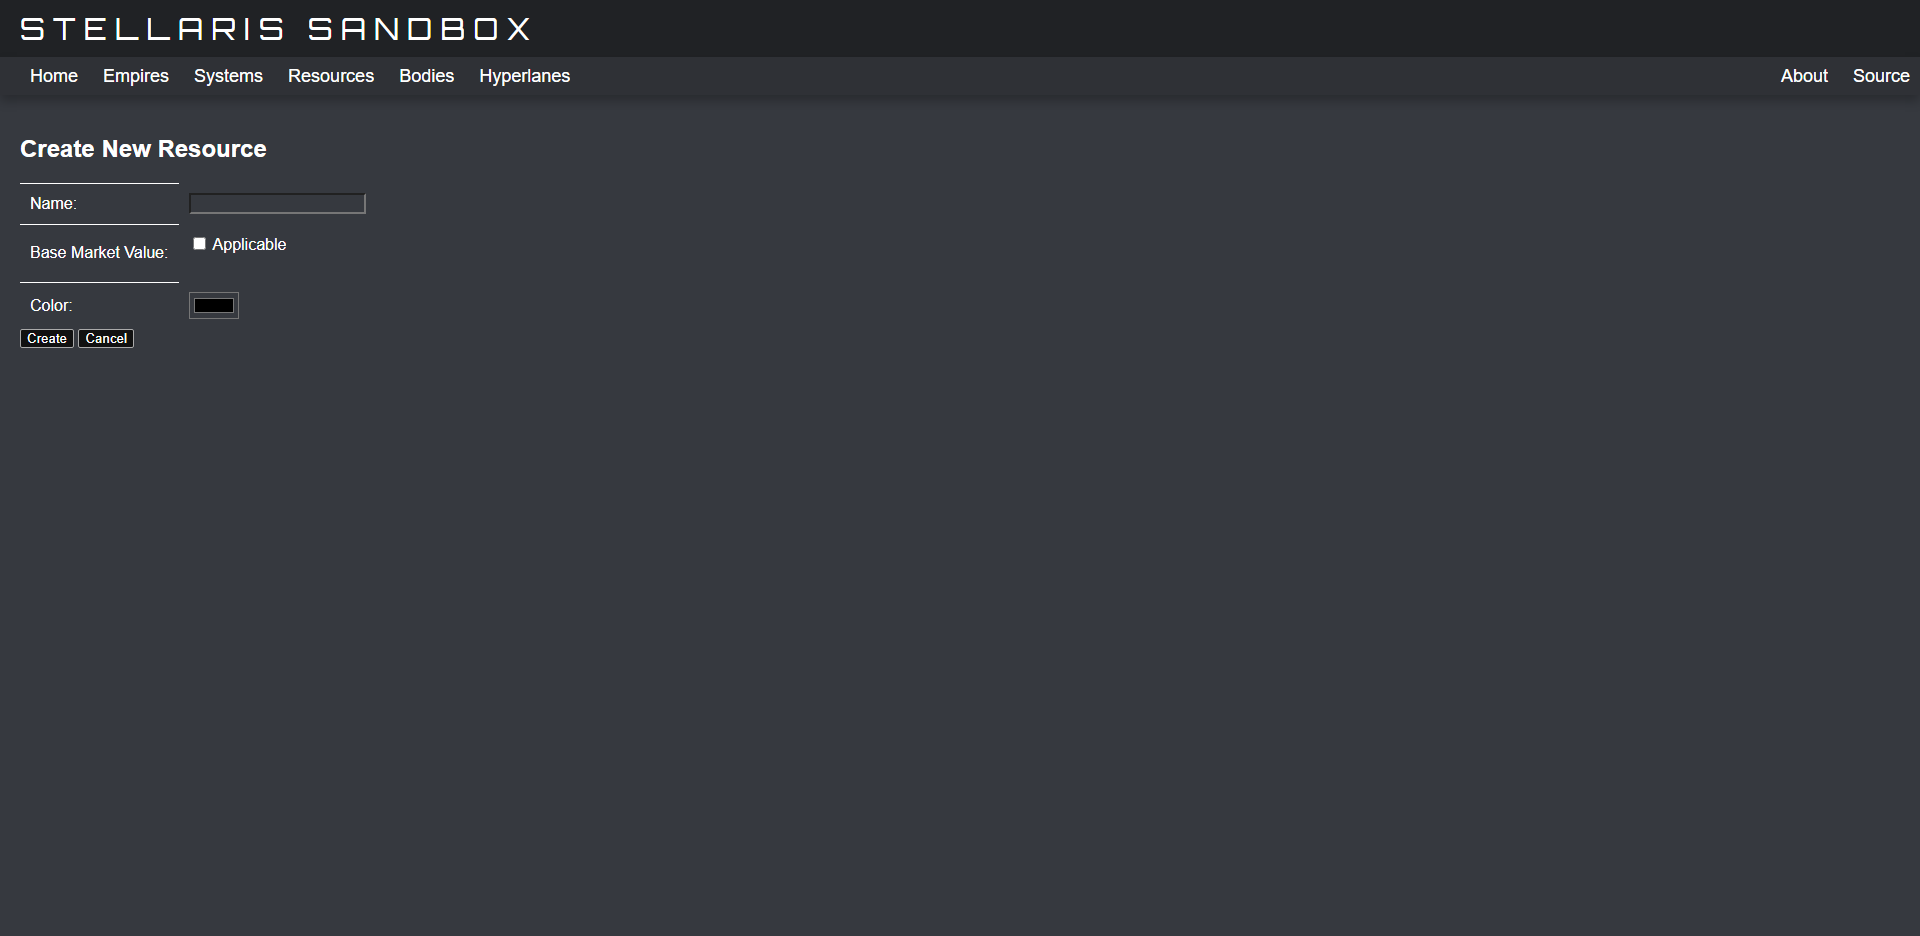
\includegraphics[width=\textwidth]{screenshots/resources/resources_create.png}
\end{figure}

\begin{figure}[!ht]
  \caption{READ Resource page.}
  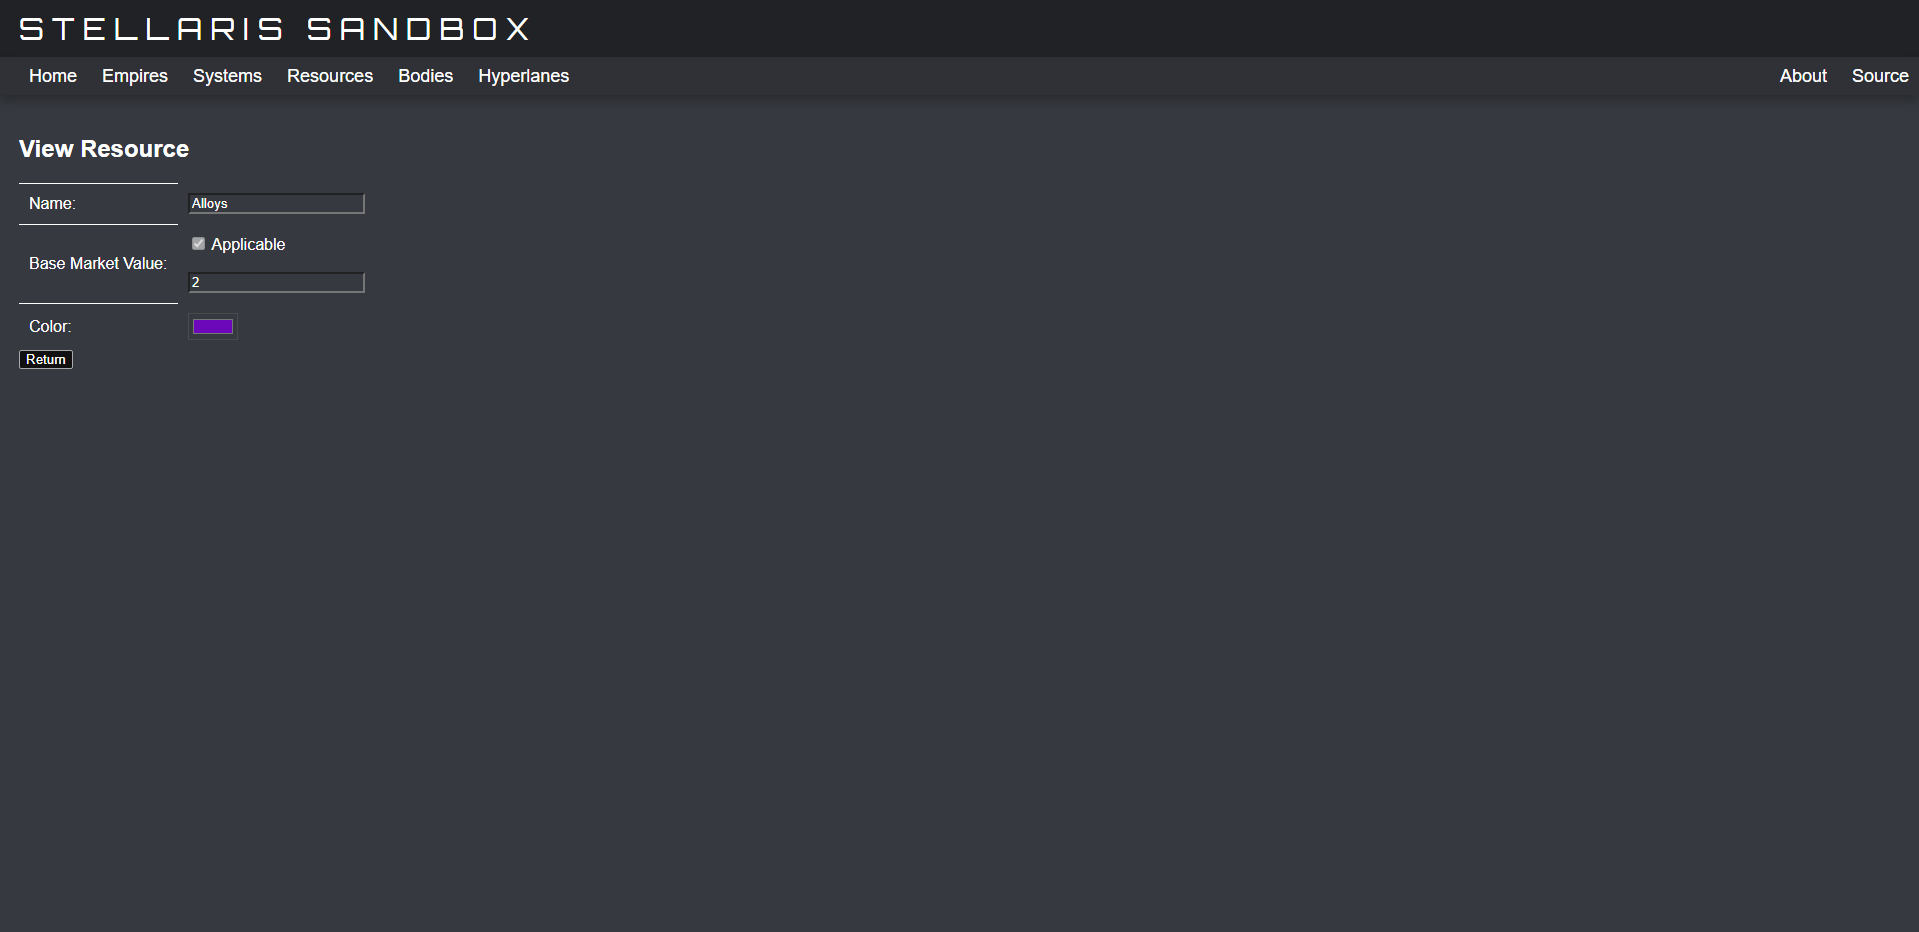
\includegraphics[width=\textwidth]{screenshots/resources/resources_read.png}
\end{figure}

\begin{figure}[!ht]
  \caption{READ/UPDATE Resource page.}
  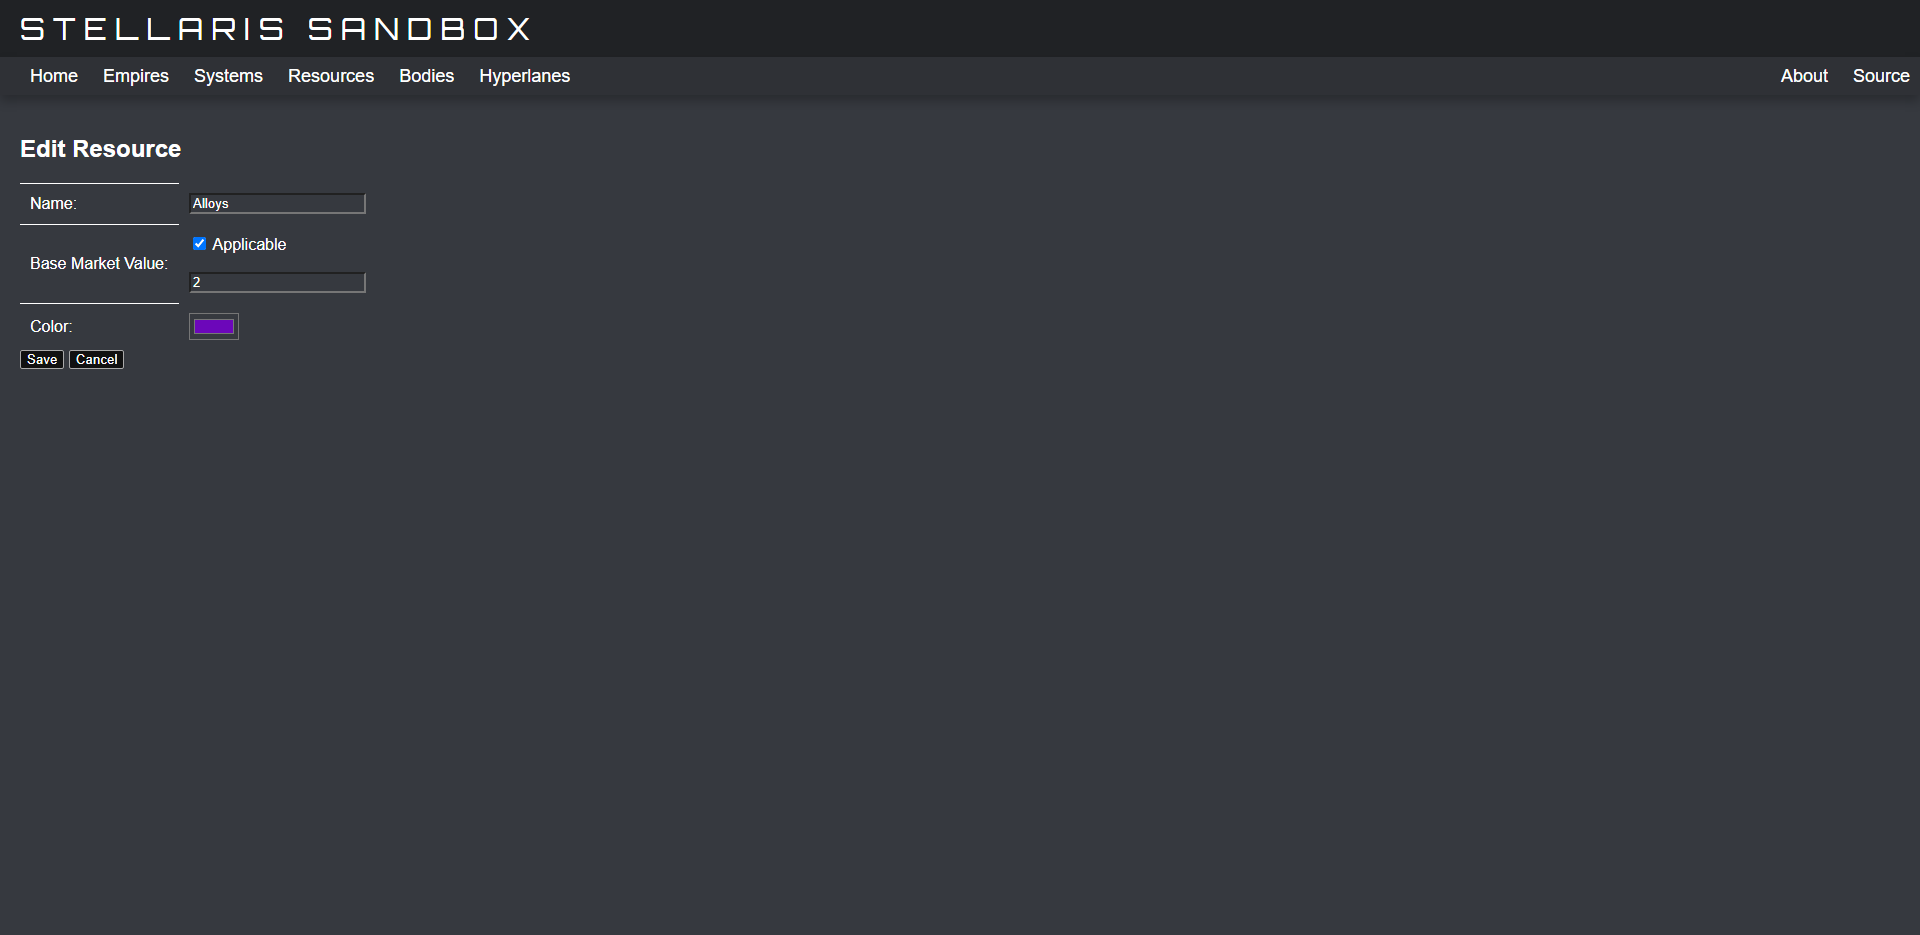
\includegraphics[width=\textwidth]{screenshots/resources/resources_read_update.png}
\end{figure}

\newpage
\subsection{Hyperlanes}

\begin{figure}[!ht]
  \caption{BROWSE/READ Hyperlanes page.}
  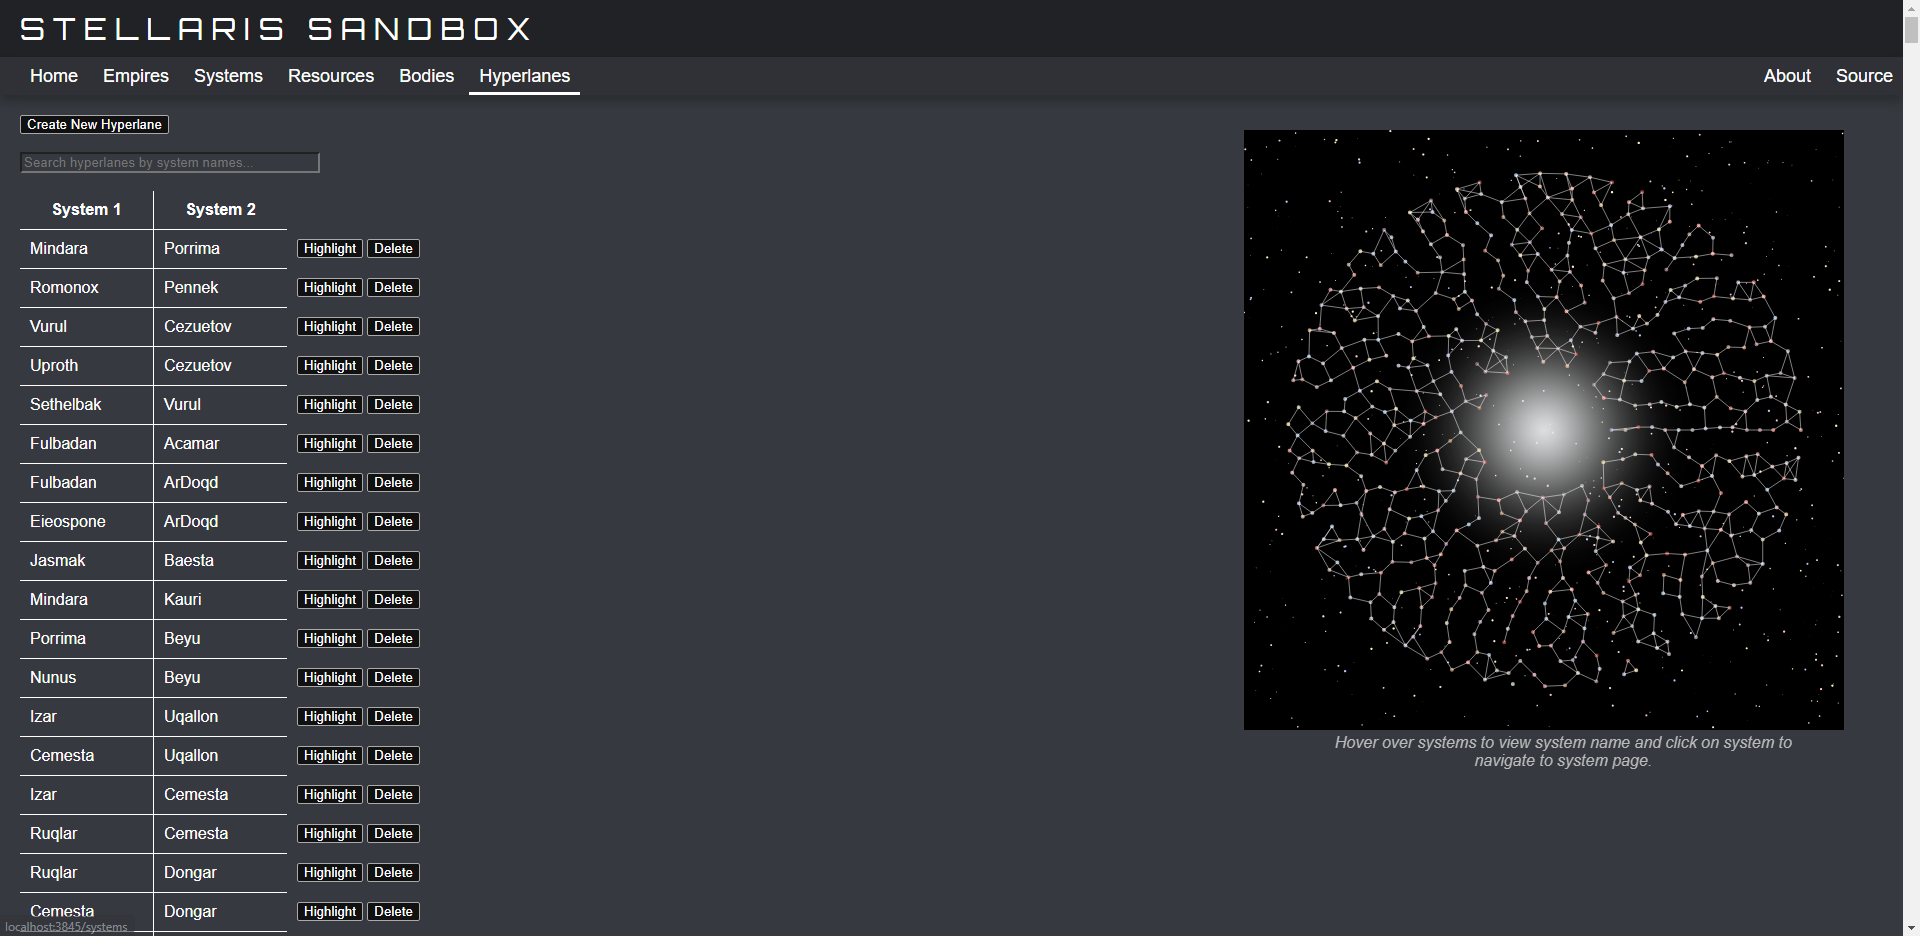
\includegraphics[width=\textwidth]{screenshots/hyperlanes/hyperlanes_browse_read.png}
\end{figure}

\begin{figure}[!ht]
  \caption{DELETE Hyperlane page.}
  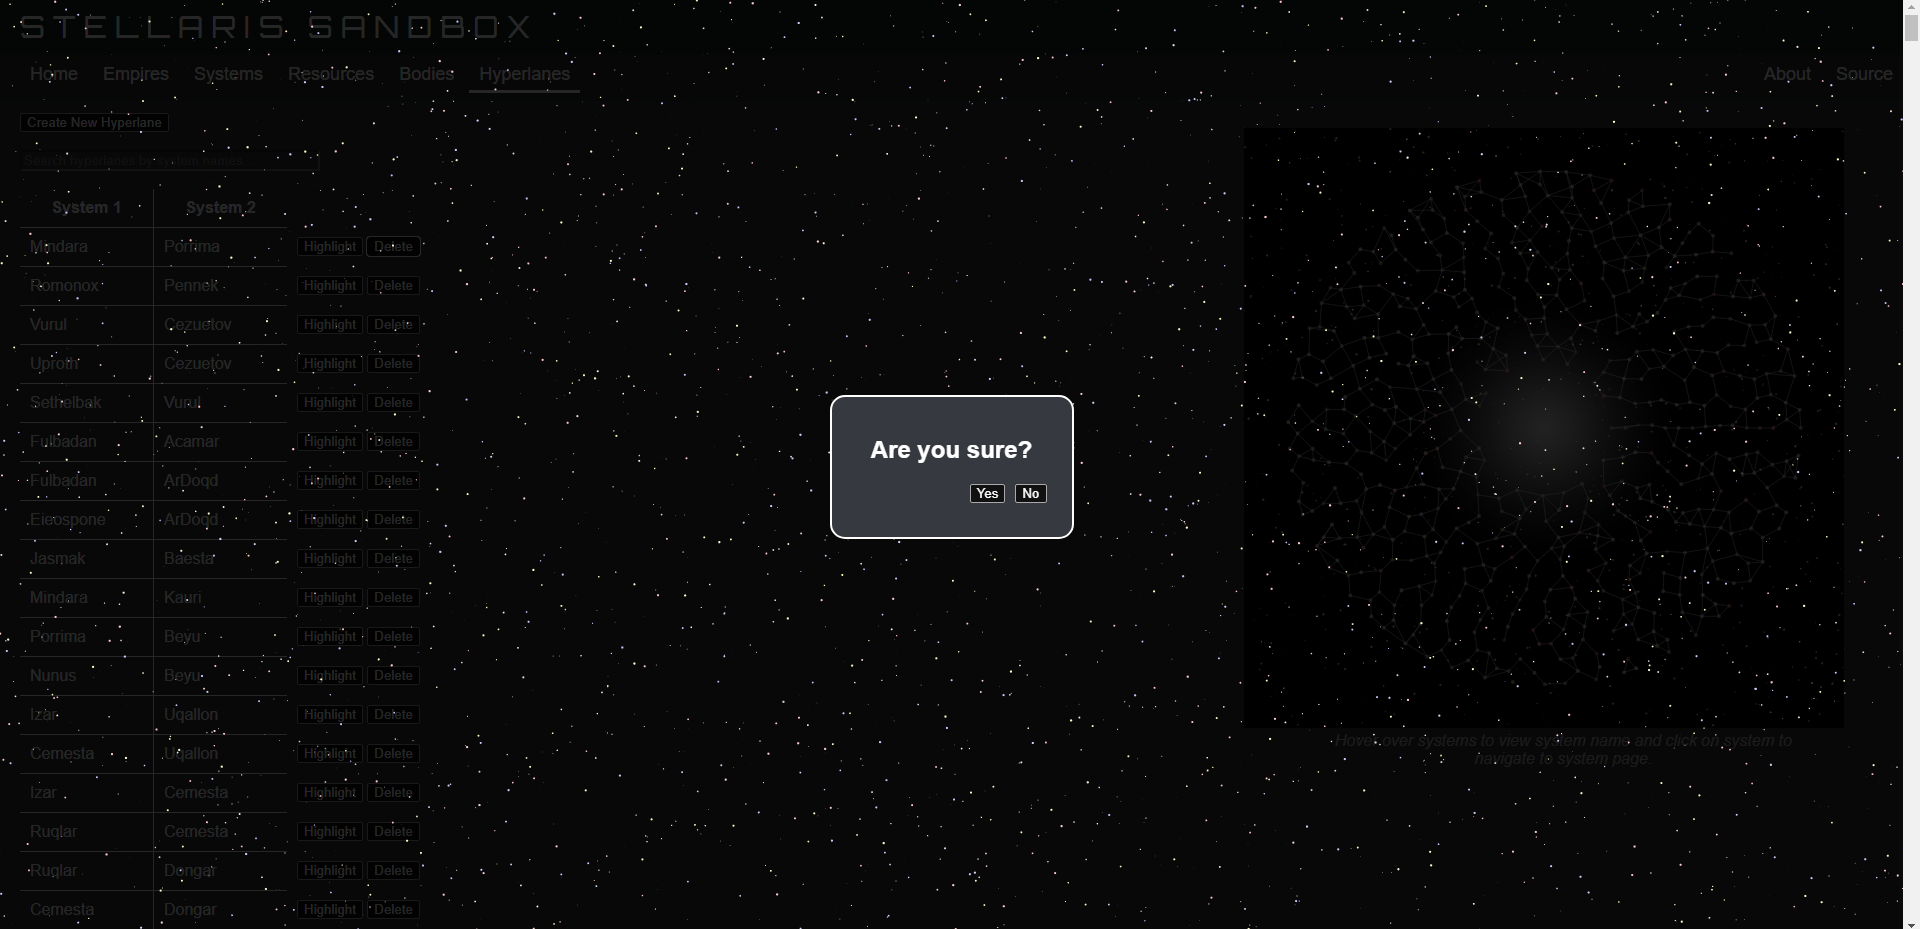
\includegraphics[width=\textwidth]{screenshots/hyperlanes/hyperlanes_delete.png}
\end{figure}

\begin{figure}[!ht]
  \caption{CREATE Hyperlane page.}
  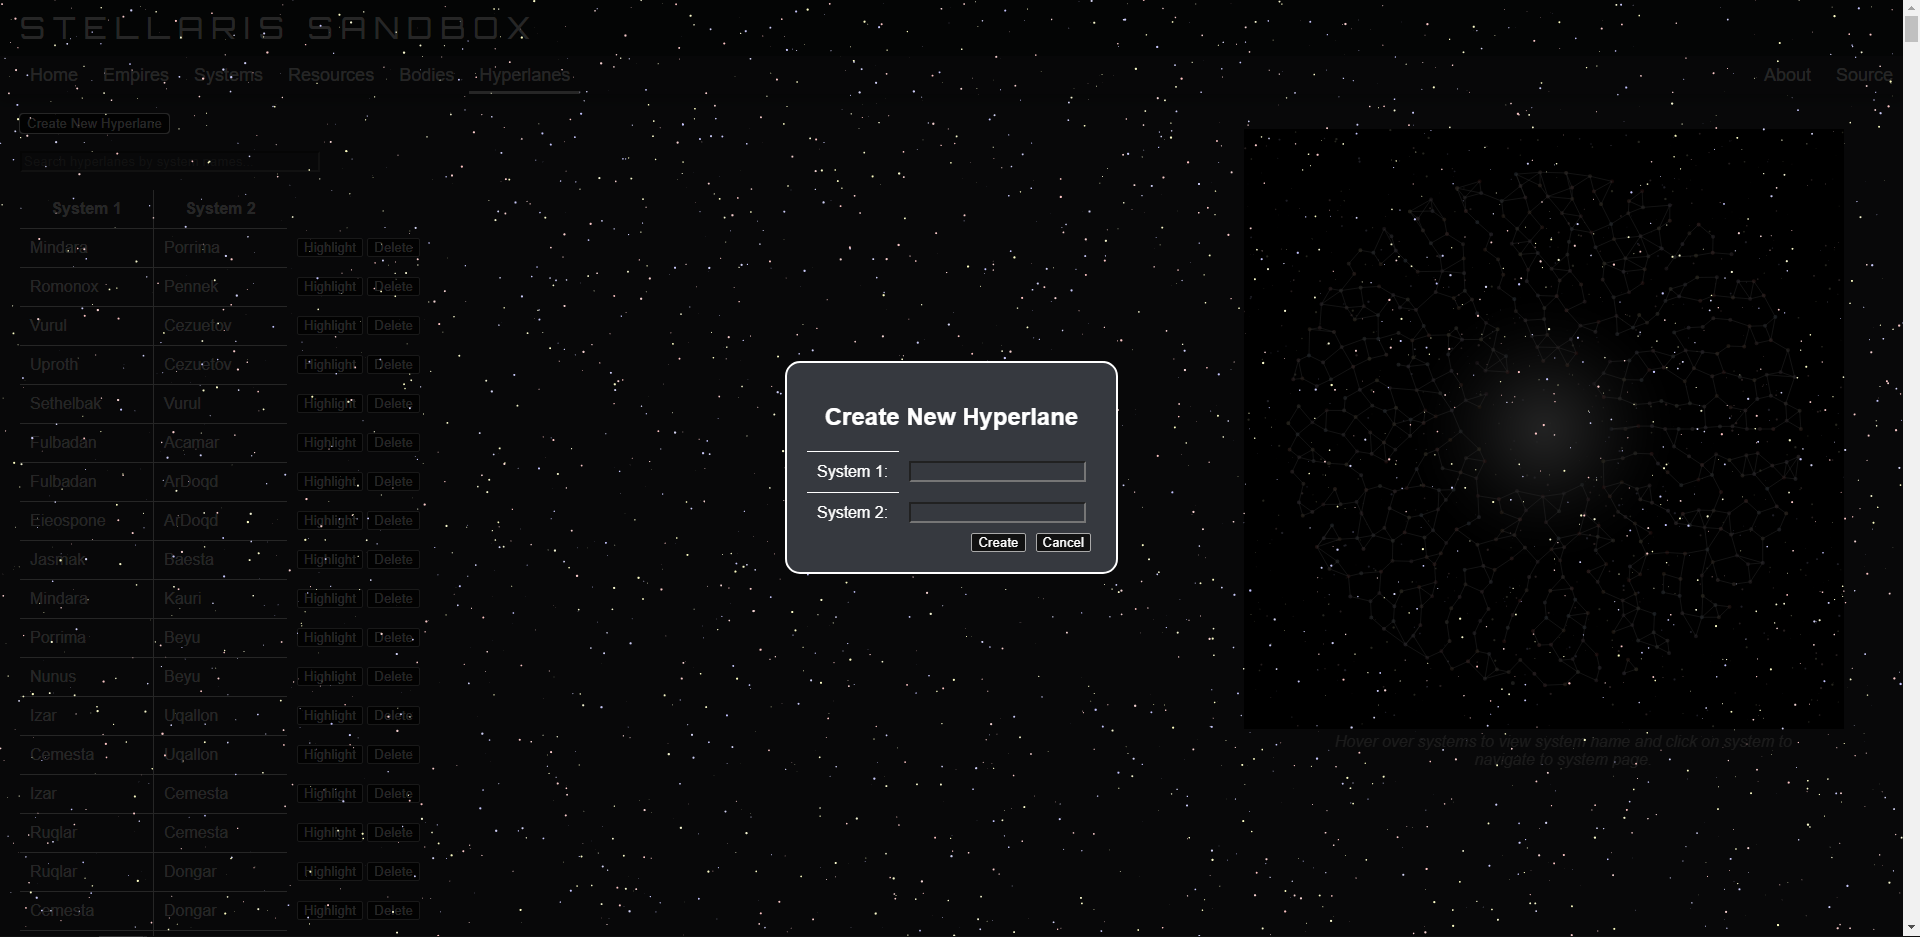
\includegraphics[width=\textwidth]{screenshots/hyperlanes/hyperlanes_create.png}
\end{figure}

\newpage
\subsection{Miscellany}

\begin{figure}[!ht]
  \caption{About page.}
  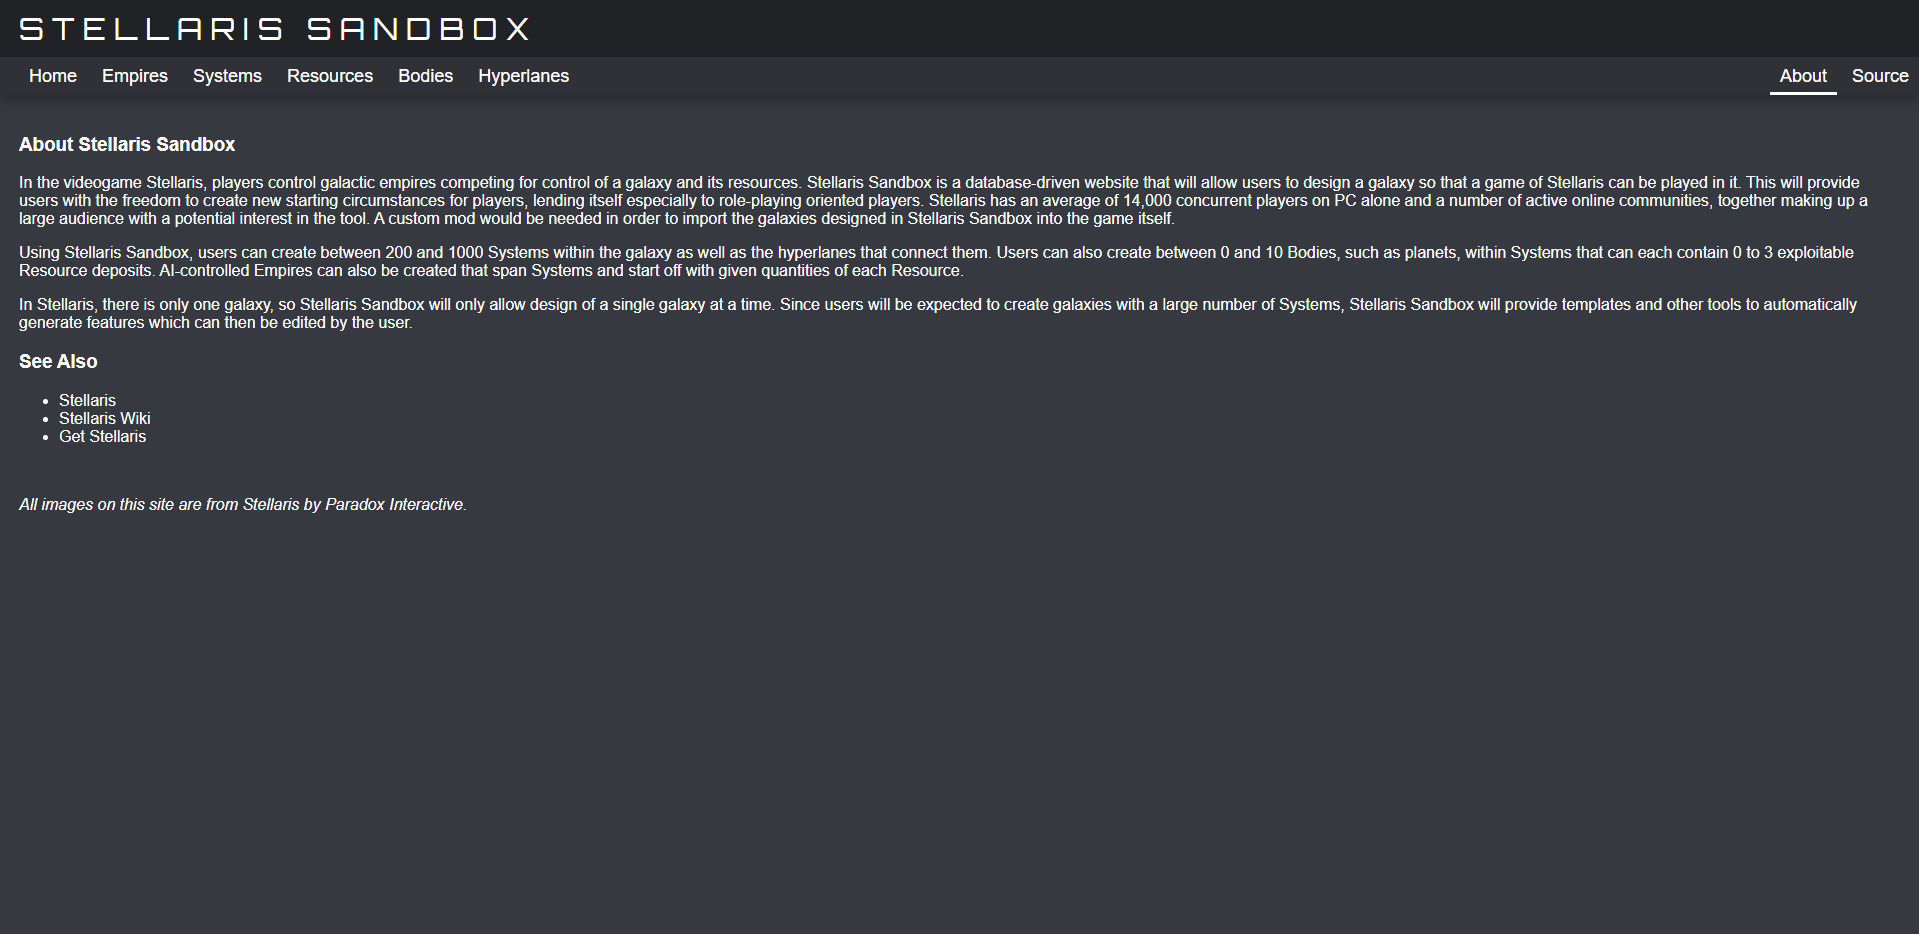
\includegraphics[width=\textwidth]{screenshots/misc/about.png}
\end{figure}

\begin{figure}[!ht]
  \caption{404 page.}
  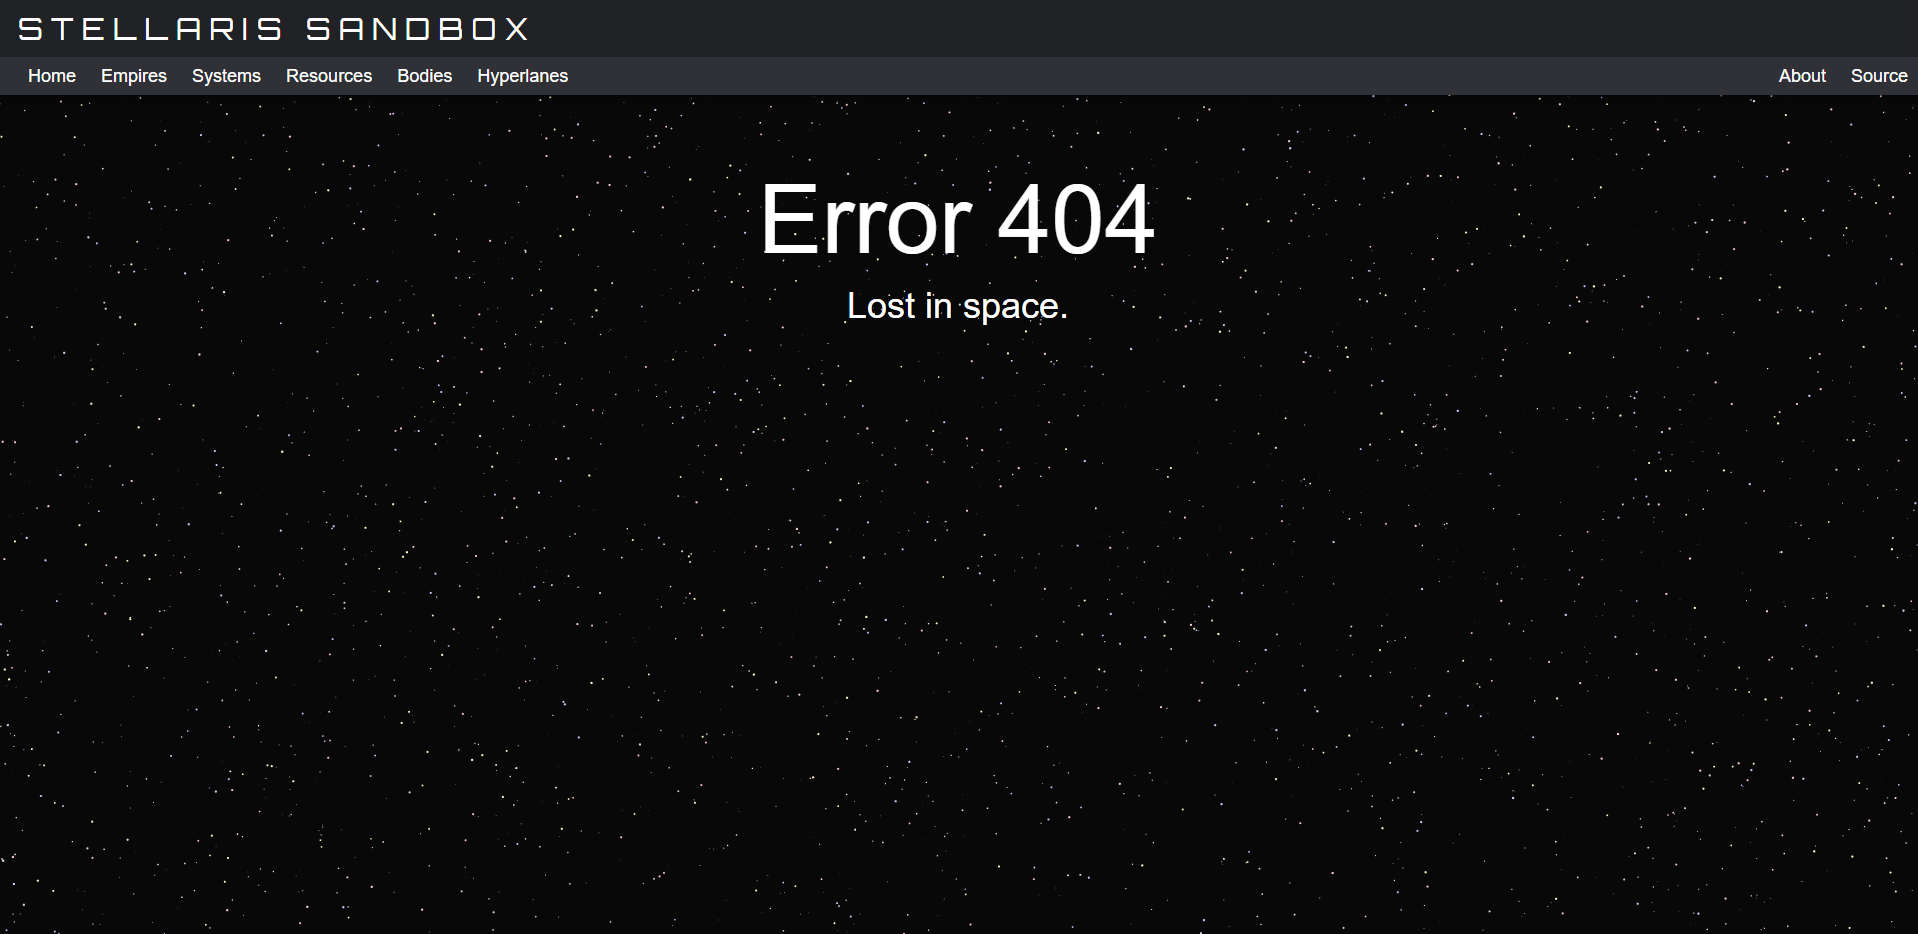
\includegraphics[width=\textwidth]{screenshots/misc/404.png}
\end{figure}

\end{document}
